%!TEX root = ../report.tex

\begin{document}

    \chapter{Supplementary}
    This chapter acts as a supplementary for the thesis.
    \section{RandLA-Net - Dropout}
    \label{sec:randladout}
    The original architecture of the RandLA-Net has only one dropout layer at the end of the second classification layer, represented as DP in Figure~\ref{fig:networkarchitecture}.
    We also used the same setup for our dropout experiment with a dropout probability of 0.5.
    Similar to other experiments, we performed 20 forward passes on the dropout, then averaged and represented every AUROC performance on every $5^{th}$ forward pass.
    \section{Summary of the models}
    As the survey of existing 3D semantic segmentation models is a part of this thesis, we display a table that summarizes the performance of each model discussed in Section~\ref{sec:dl_approach}.
    \begin{longtable}{|p{0.15\linewidth} | p{0.59\linewidth}| p{0.06\linewidth} |p{0.09\linewidth}|}
        %\centering
        %\begin{tabular}{|p{0.15\linewidth} | p{0.6\linewidth}| p{0.06\linewidth} |p{0.08\linewidth}|}
            \hline
            \textbf{Method} & \textbf{Summary} & \textbf{Type} & \textbf{\#Params} \\
            \hline 
            PointNet\cite{Qi_2017_CVPR_pointnet} &
            PointNet works on raw point cloud and acheives permutation invariance of point cloud by using maxpooling as symmetric function.
            Transformation invariance of point cloud is acheived by generating a transformation matrx generated by Spatial Transformer Network.
            gloabl features are extracted by maxpooling layer and fed into segmentation head for 3D segmentation.
            & Point & 3M \\
            \hline
            PointNet++\cite{qi2017pointnet++} &
            PointNet doesnt capture local structures becuase of only global features extraction.
            So PointNet++ applies PointNet recursively on portions of input point cloud to extract featuers and these are grouped to form high level features.
            & Point & 6M \\
            \hline
            TangentConv\cite{Tatarchenko_2018_CVPR_tangconv} &
            Proposes tangent convolutions which are simialr to normal convolution but an additional multiplication of gaussian kernel.
            The architecture is encoder-decoder style with fully convolutional network consisting of tangent convolutions.
            & Point & 0.4M\\
            \hline
            SPLATNet\cite{Su_2018_CVPR_splatnet} &
            This model uses Bilateral Convolutional Layers(BCL) to project data onto low dimensional lattice.
            These lattices from BCL are then convolved and reprojected back to the point cloud.
            USe of BCL allows the projection 2D semantic labels to label the 3D point cloud.
            & Point & 0.8M \\
            \hline
            SqueezeSeg\cite{Sequeseseg_2018} &
            Projects the data onto 2D spherical coordinates and segmented using SqueezeNet.
            The segmented 2D image is reprojected back to 3d using Recurrent Conditional Random Fields.
            & Project & 1M \\
            \hline
            SqueezesegV2\cite{SqueezeSegv2} &
            Extension over SqueezeSeg by using Context Aggregation Module (CAM) before encoder to minimize the effects of missing points on convolutional filters of SqueezeSeg.
            Proposed novel focal loss instead of weighted cross entropy to better represent the dataset class imbalance.
            & Project & 1M \\
            \hline
            SqueezesegV3\cite{xu2020squeezesegv3} &
            Spherical proejction based model which uses Spatially Adaptive Convolutions to change filters according to the differnt locations in the input image.
            The architecture is similar to RangeNet with cross entropy loss calculated at each layer.
            & Project & 0.92M \\
            \hline
            %SPGraph\cite{SPGraph} & & Point & 0.25M\\
            %\hline
            LatticeNet\cite{rosu2019latticenet}\footnote{LatticeNet has no code to calculate number of parameters.} &
            The input point cloud is projected onto d-dimensional sparse lattice and reprojection is learnt form the data by using novel proposed DeformSlice module.
            The architecture is similar to U-Net with lattice projeciton at encoder and DeformSlice at end of decoder module.
            & Point & - \\
            \hline
            RangeNet-21\cite{Milioto2019} & 
            Spherical projection based model with encoder-decoder style architecture with encoder being DarkNet21.
            Introduced a better evaluation metric called borderIoU for occlusions.
            & Project & 25M \\
            \hline
            RangeNet-53\cite{Milioto2019}  & 
            Architecturally similar to RangeNet-21, the only change is encoder which is DarkNet53.
            No postprocessing is applied for occlusions or nonprojected points.
            & Project & 50M \\
            \hline
            RangeNet-53++\cite{Milioto2019} &
            RangeNet-53++ architecture is same as RangeNet-53 but a post processing 
            method of kNN is applied on output to label the occluded points or nonprojected points after reprojection from segmented 2D spherical image to 3D points.
            & Project & 50M \\
            \hline
            RandLA-Net\cite{Hu_2020_CVPR_Randla} & 
            Random points from input point cloud are sampled and fed into local feature aggregation (LFA) module for feature extraction.
            These fetures are weighted and selected based on the attention score. 
            Encoder-decoder style architecture with stacks of LFA as encoder and decoder is transponse convolutions for upsampling with MLP followed by fully connected layers for segmentation.
            & Point & 0.95M \\
            \hline 
            3DMiniNet\cite{3Dmininet} &
            This model works on spherical projection of 3D point cloud which is fed into projection learning module to learn local and global features.
            These learnt features are fed into MiniNetV2 which is a fully connected neural network for segmentation of spherical image.
            This 2D image is reprojected back into 3D point cloud using kNN search as in RangeNet53++.
            & Project & 4M \\
            \hline
            SalsaNet\cite{salsanet2020} & Encoder-decoder style architecture with Bird-Eye-View projection as input and encoder consisting of ResNet blocks and decoder with transpose convolutions.
            Unlabelled points in LiDAR are auto labelled from corresponding images. Claims SalsaNet is projection agnostic.
            & Project & 6.6M \\
            \hline
            SalsaNext\cite{SalsaNext_2020} & 
            Similar architecture to SalsaNet, proposed a new context module replacing ResNet module in encoder and pixel shuffle instead of transposed convolutions in decoder.
            Proposed Lovasz-Softmax loss in combination with weighted cross-entropy loss.
            This is the first model best of our knowledge to study epistemic and aleatoric uncertainty by modelling SalsaNext as Bayesian Neural Network.
            & Project & 6.7M \\
            \hline
            PolarNet\cite{polarnet} &
            It is a projection based model, instead of spherical or bird's eye view projection in cartesian coordinate system, this model projects the data into bird's eye view projection on to a grid of polar coordinate system.
            This grid is a fixed size representation and features are extracted are for each grid cell.
            & Project & 14M \\
            \hline
            KPRNet\cite{kochanov2020kprnet} &
            Projects the data into 2D spherical image and 2D CNN encoder-decoder architecture is applied.
            Encoder consists of ResNeXt-101 and decoder is similar to DeepLab with depthwise seperable convolutions.
            Backprojection to 3D is made using KPConv similar to KNN in RangeNet-53++.
            & Project & 243M \\
            \hline
            SPVNAS\cite{spvnas} &
            Proposes Sparse Point-Voxel Convolutions (SPVConv) aimed to improve performance over small objects such as pedestrains, cyclistis.
            SPVConv voxelizes point cloud and apply sparse convolution and then devoxelizes the voxel to point cloud.
            This is the first 3D semantic segmentation model to utlize Neural Architecture Search (NAS).
            & Point & 2.6M \\
            \hline
            Cylinder3D\cite{zhu2020cylindrical}\footnote{Cylinder3D uses Sparse Convolutions which is not supported in Ubuntu-20 at the time of study. So parameters cannot be calculated.} &
            Converts 3D cartesian coordinates to 3D cylinder coordinates then voxelizes and fed into Asymmetric Residual Block to extarct these cuboid features.
            These features are applied to 3D U-Net for segmentation.
            & Project & - \\
            \hline
            %(AF)2-S3Net\cite{af2s3net} & & Point & - \\
            %\hline
            \caption{Summary of various point and projection based 3D semantic segmentation models. In Type column point represent point based model and project represents projection based model.}
            \label{tab:model_relatedwork}
        %\end{tabular}
    \end{longtable}
    
    \section{ROC curves}
    \label{sec:app_roc_curves}
    In this section, we display the ROC curves associated with the AUROC score from Table~\ref{tab:sem3dvs3dis_auroc}.
    Figure~\ref{fig:roc_msp_ood_1} represents the ROC curves generated using Maximum Softmax Probability (MSP) for Deep Ensembles, Flipout and Dropout.
    Similarly Figure~\ref{fig:roc_ent_ood_1} represents the ROC curves generated using the entropy score.
    In both the cases, we observe that Dropout performs near to random classifier and Deep Ensembles outperform all the other methods.

    Similarly, for Semantic3D and Semantic3D without colour, ROC curves have been depicted, and these are associated with Table~\ref{tab:auroc_ood_2}.
    Figure~\ref{fig:roc_msp_ood_2} and Figure~\ref{fig:roc_ent_ood_2} represents the ROC curves generated using MSP and entropy respectively.
    In the case of MSP depicted in Figure~\ref{fig:roc_msp_ood_2}, we observe Deep Ensembles outperform other methods.
    Whereas in the case of entropy depicted in Figure~\ref{fig:roc_ent_ood_2}, we observe similar overlapping ROC curves between Deep Ensembles, Flipout and Dropout.
    \begin{figure*}
        \centering
        \begin{tabular}{cc}
            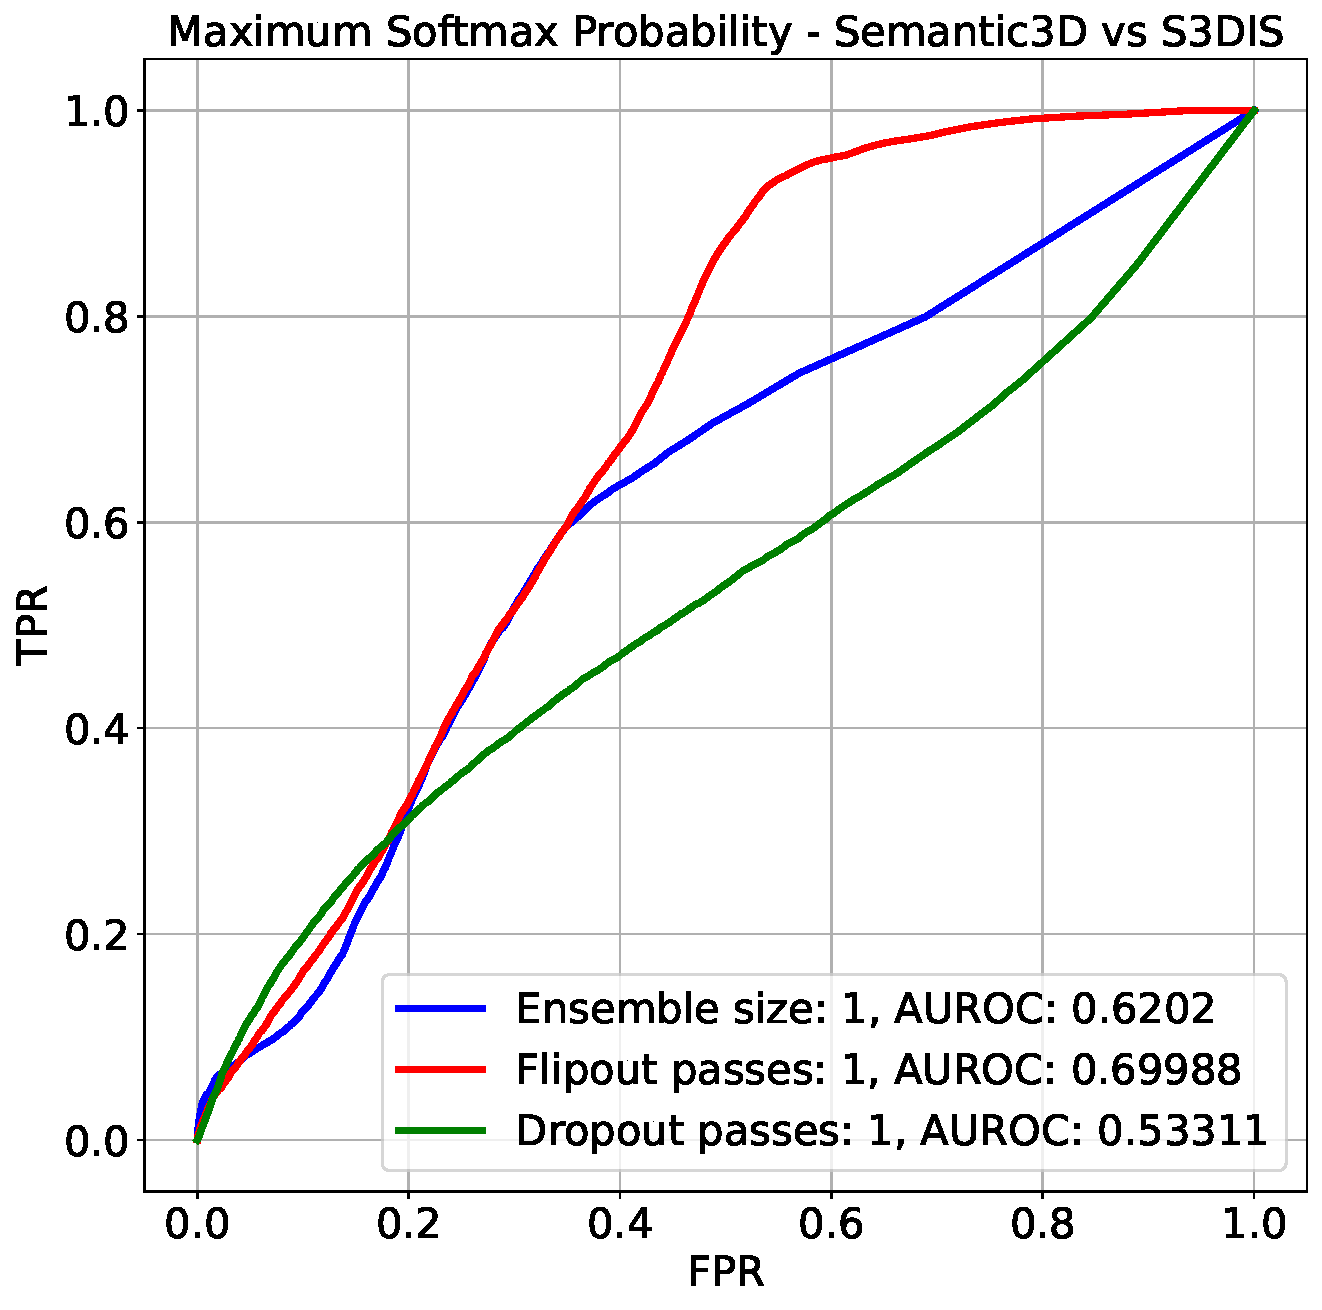
\includegraphics[width = 0.42\textwidth, height= 0.3\textheight]{images/AUROC/MSP_1.pdf} & 
            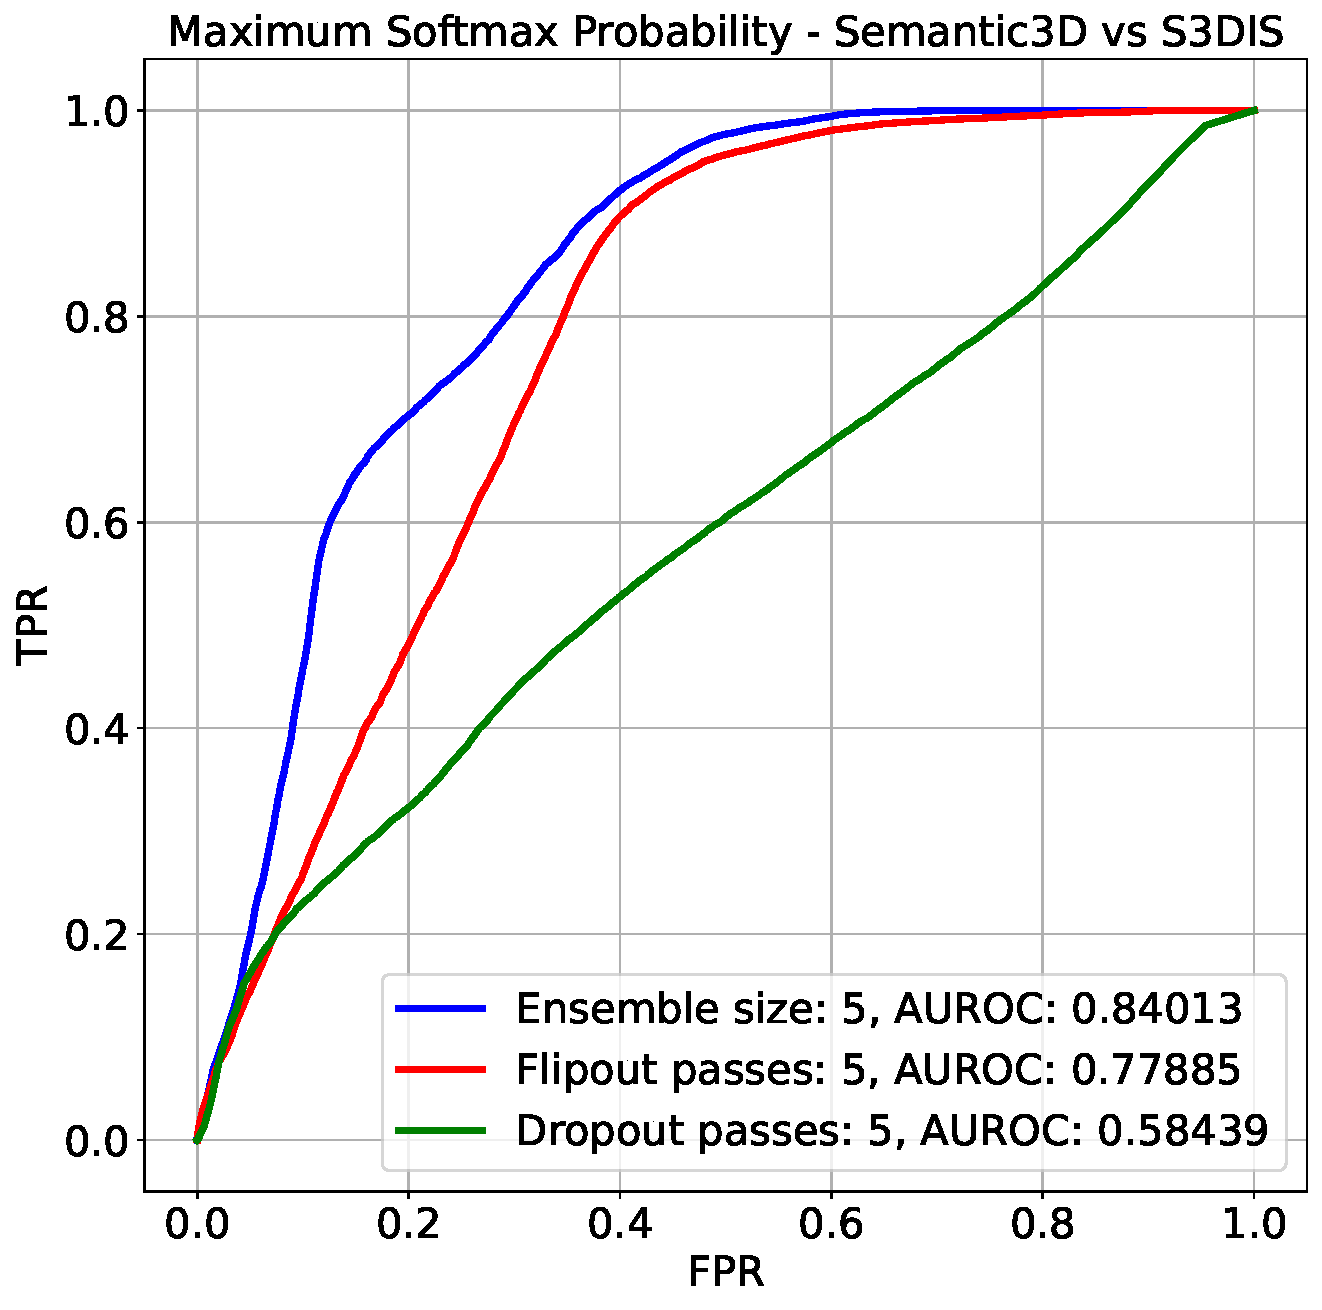
\includegraphics[width = 0.42\textwidth, height= 0.3\textheight]{images/AUROC/MSP_5.pdf}\\ 
            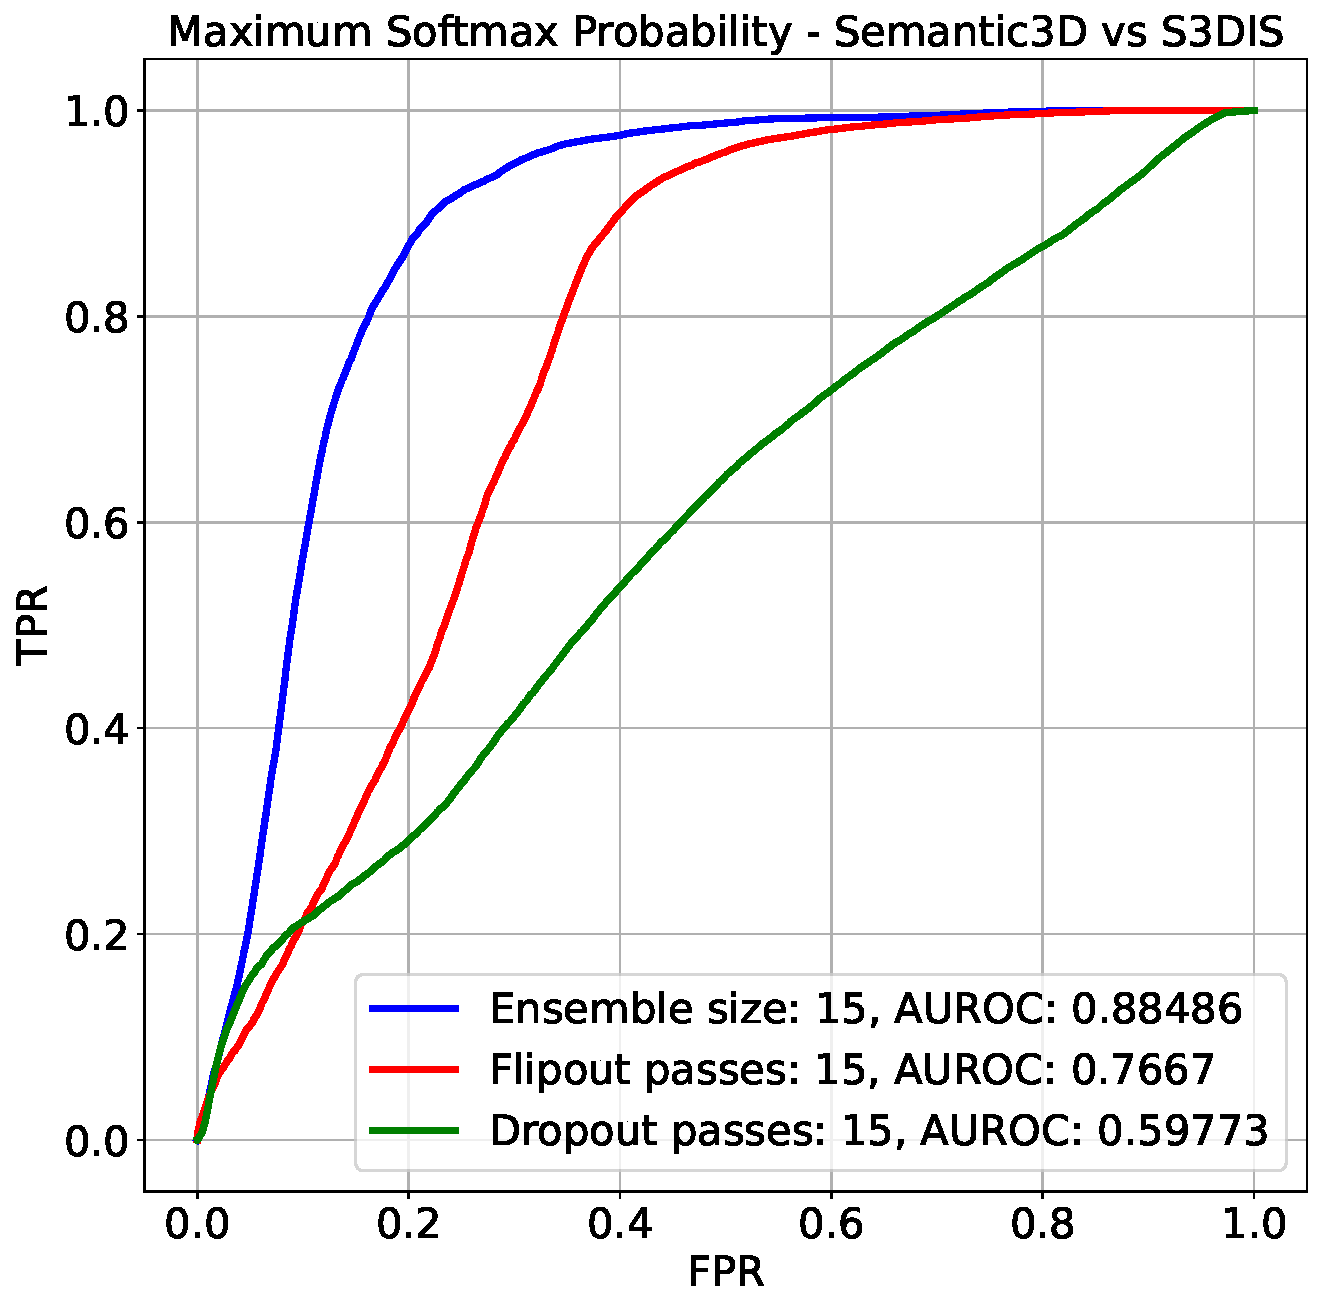
\includegraphics[width = 0.42\textwidth, height= 0.3\textheight]{images/AUROC/MSP_15.pdf} & 
            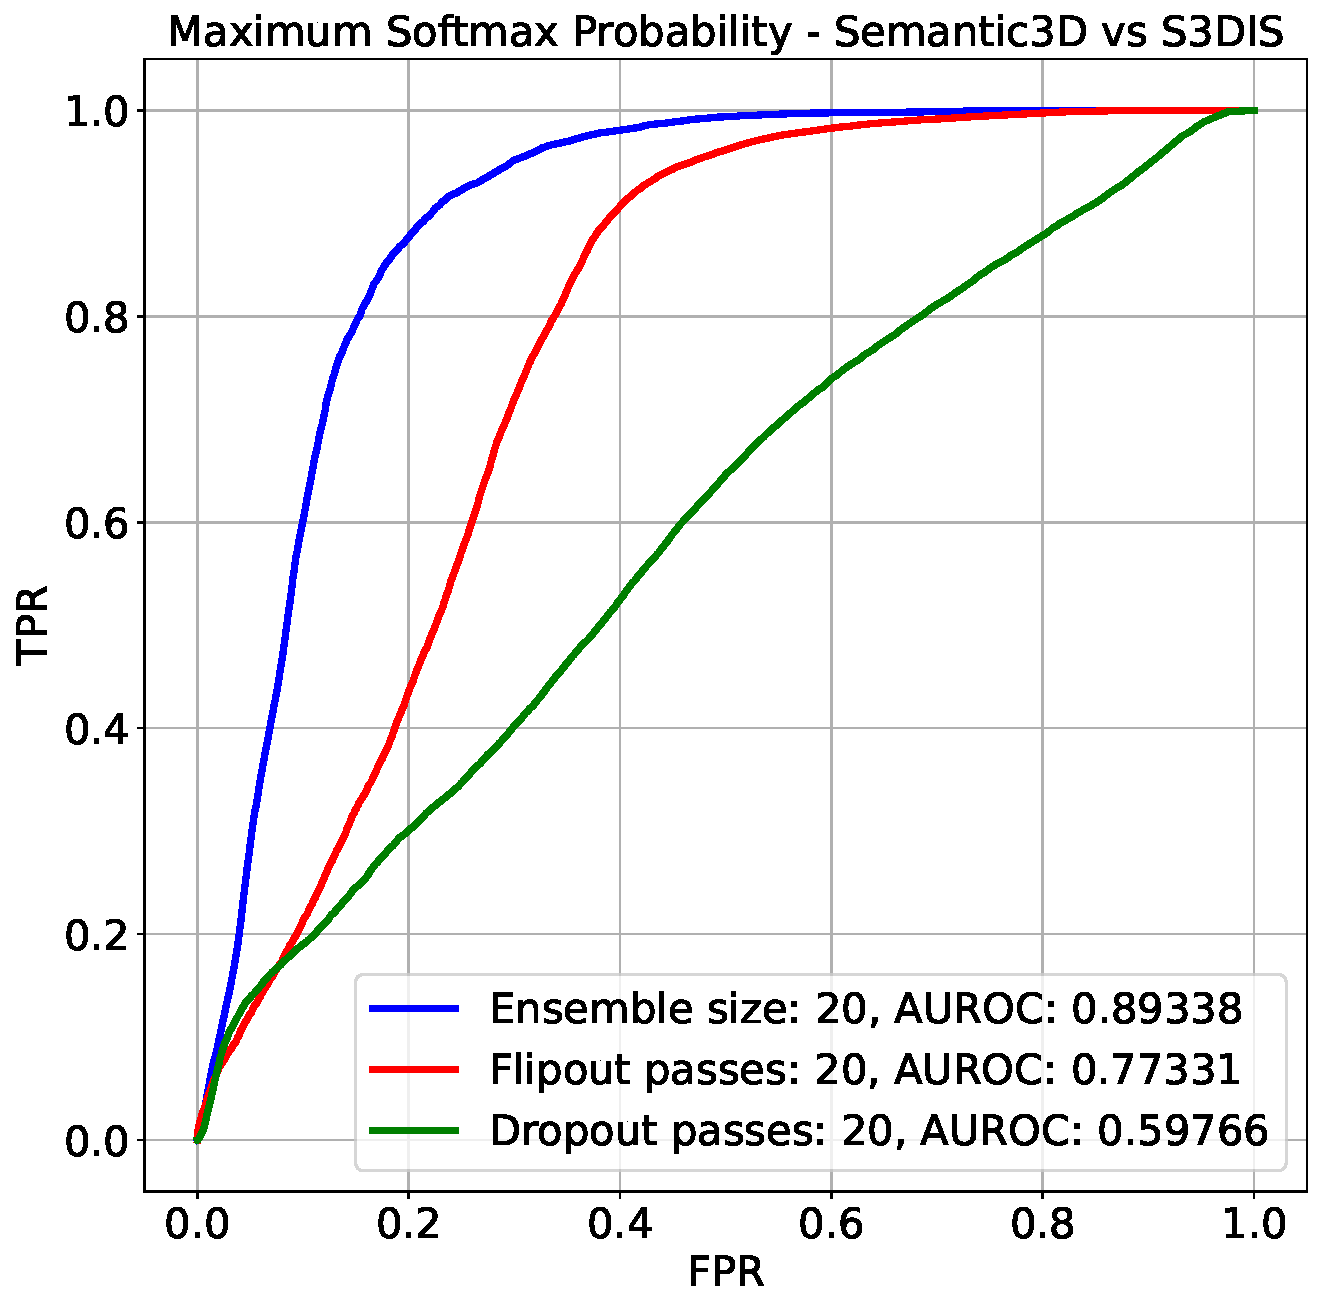
\includegraphics[width = 0.42\textwidth, height= 0.3\textheight]{images/AUROC/MSP_20.pdf} \\
        \end{tabular}
        \caption{ROC curves for Semantic3D vs S3DIS generated using Maximum Softmax Probability for Deep Ensembles, Flipout and Dropout.}
        \label{fig:roc_msp_ood_1}
    \end{figure*}
    \begin{figure*}
        \centering
        \begin{tabular}{cc}
            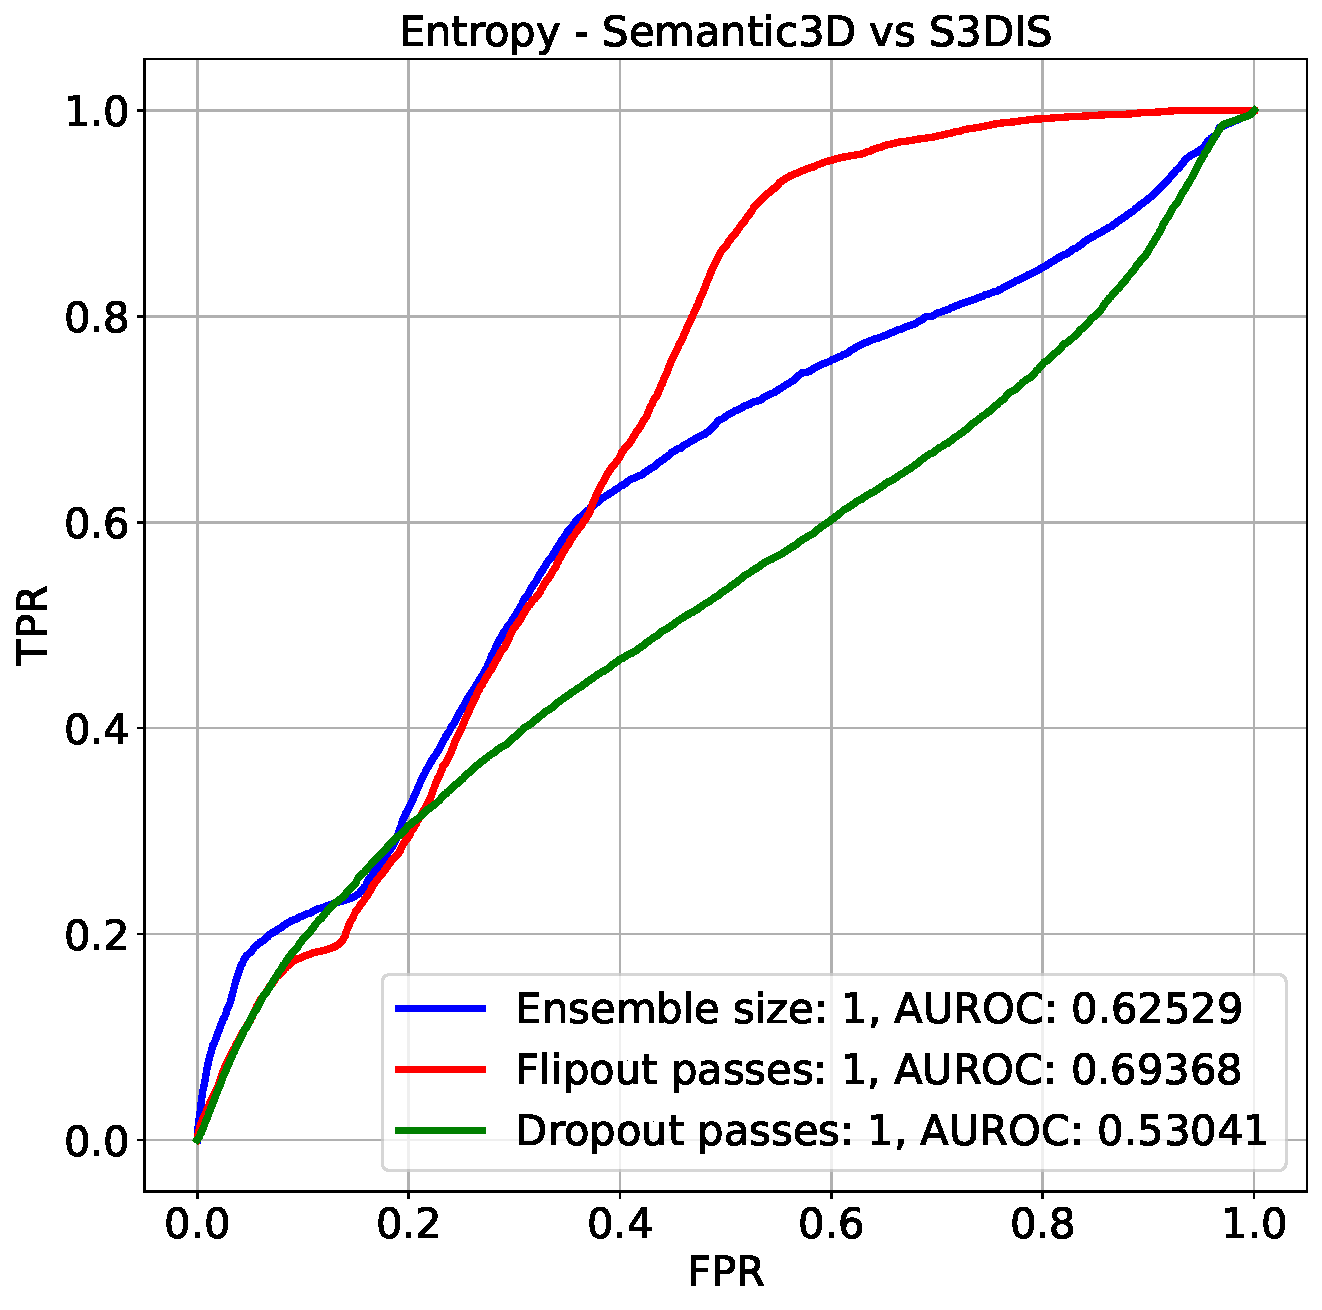
\includegraphics[width = 0.42\textwidth, height= 0.3\textheight]{images/AUROC/Entropy_1.pdf} & 
            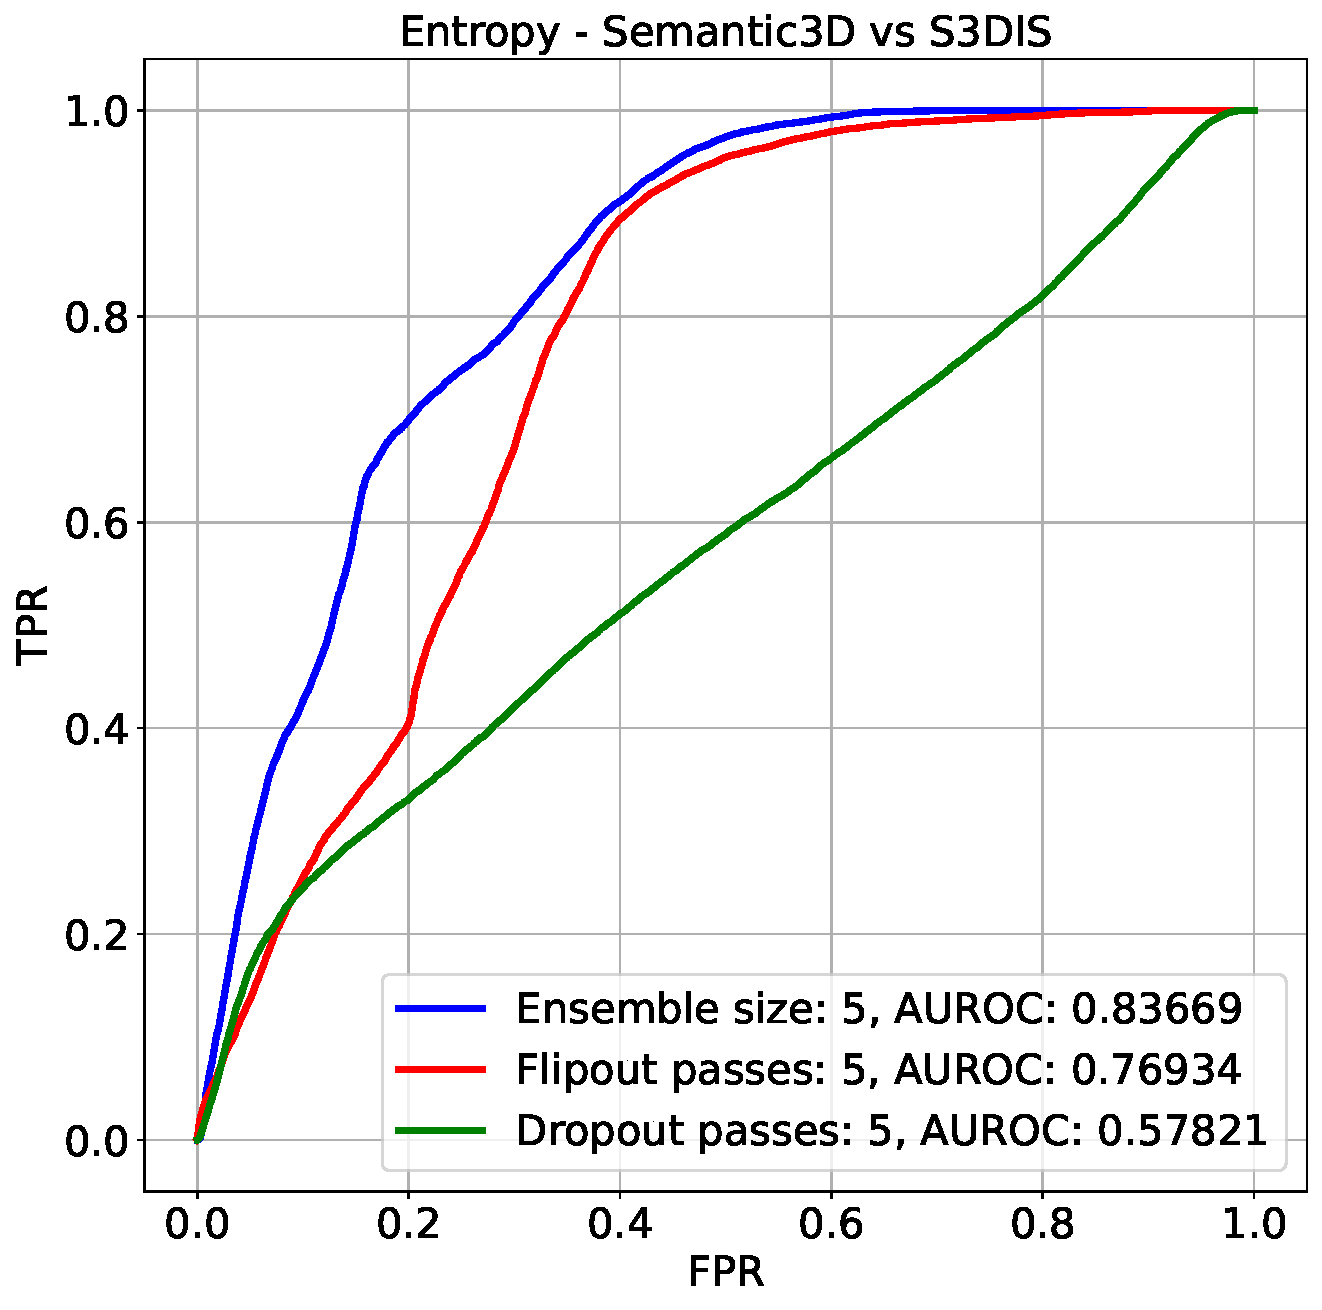
\includegraphics[width = 0.42\textwidth, height= 0.3\textheight]{images/AUROC/Entropy_5.pdf}\\ 
            
            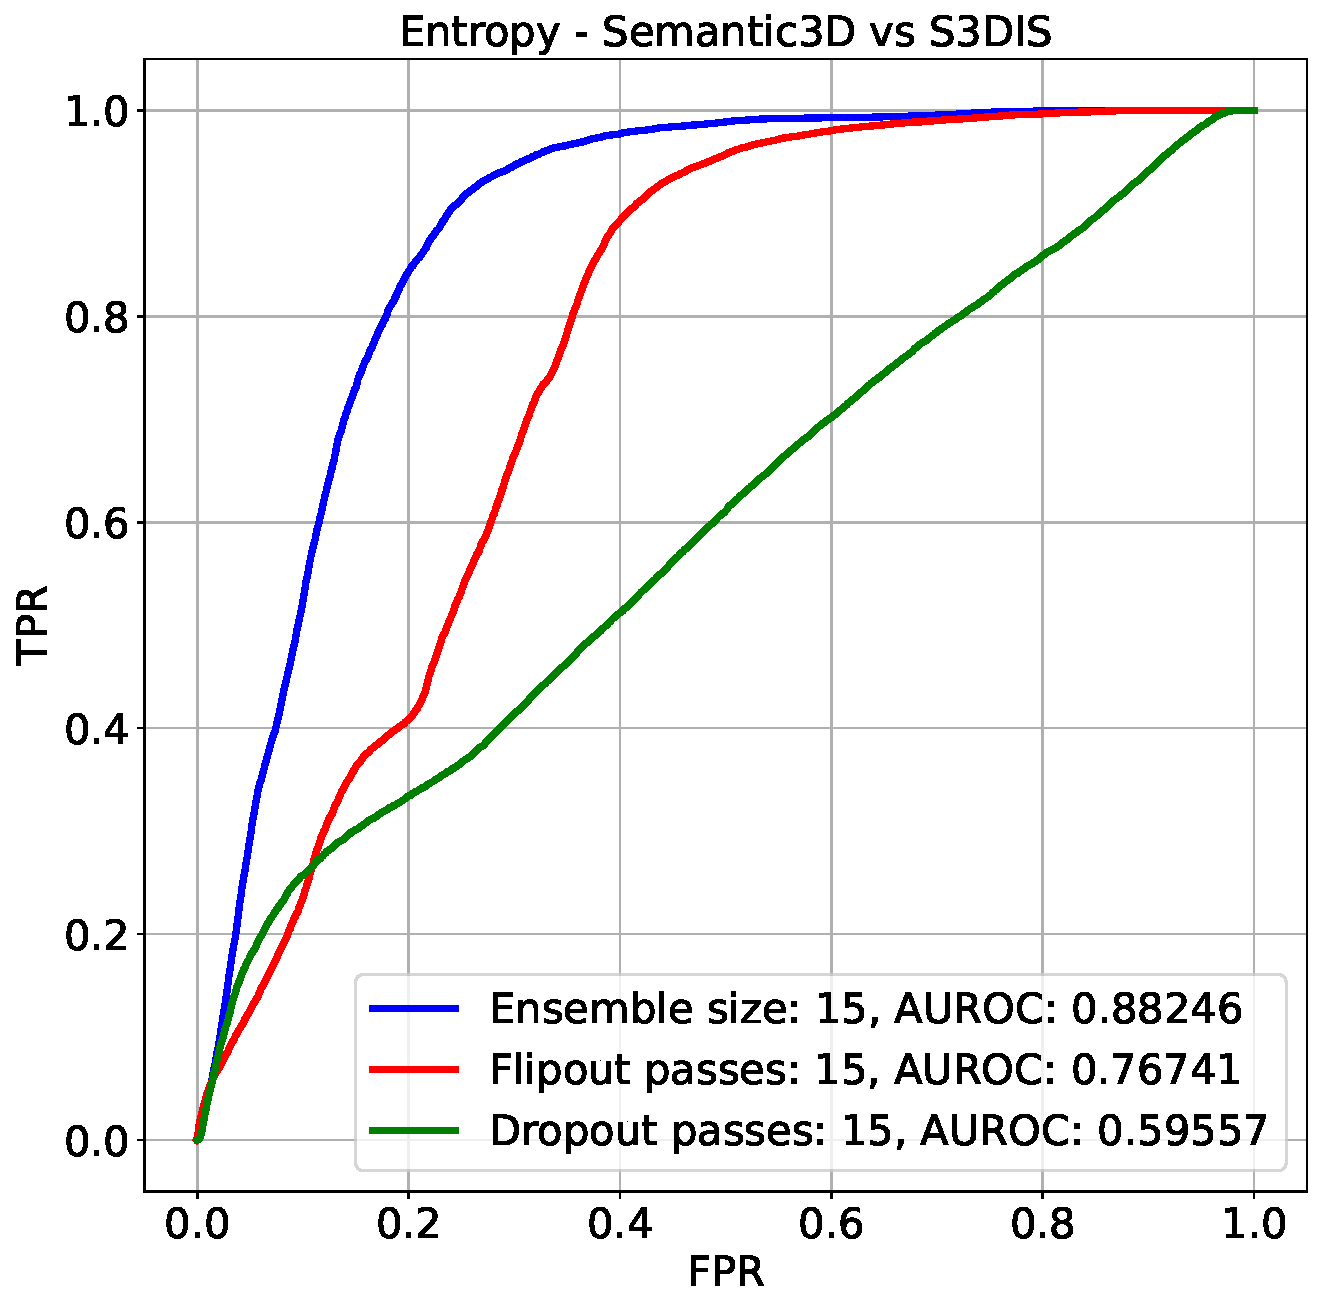
\includegraphics[width = 0.42\textwidth, height= 0.3\textheight]{images/AUROC/Entropy_15.pdf} &
            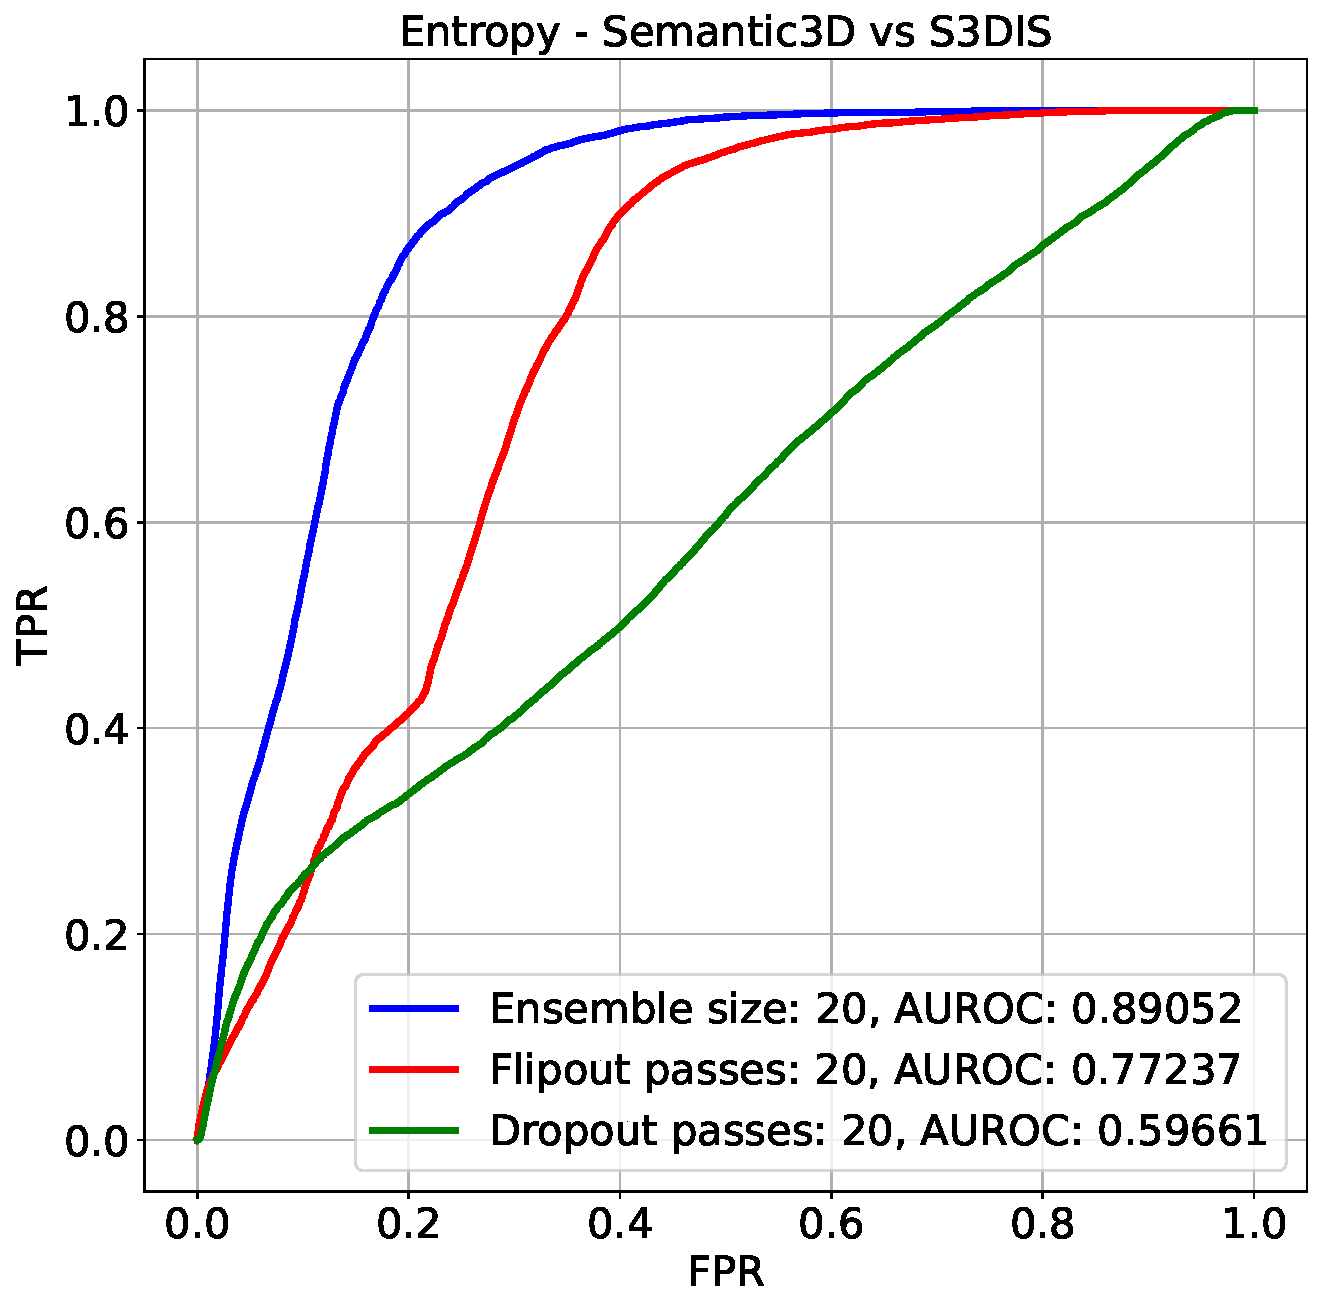
\includegraphics[width = 0.42\textwidth, height= 0.3\textheight]{images/AUROC/Entropy_20.pdf} \\
        \end{tabular}
        \caption{ROC curves for Semantic3D vs S3DIS generated using Entropy for Deep Ensembles, Flipout and Dropout.}
        \label{fig:roc_ent_ood_1}
    \end{figure*}

    \begin{figure*}
        \centering
        \begin{tabular}{cc}
            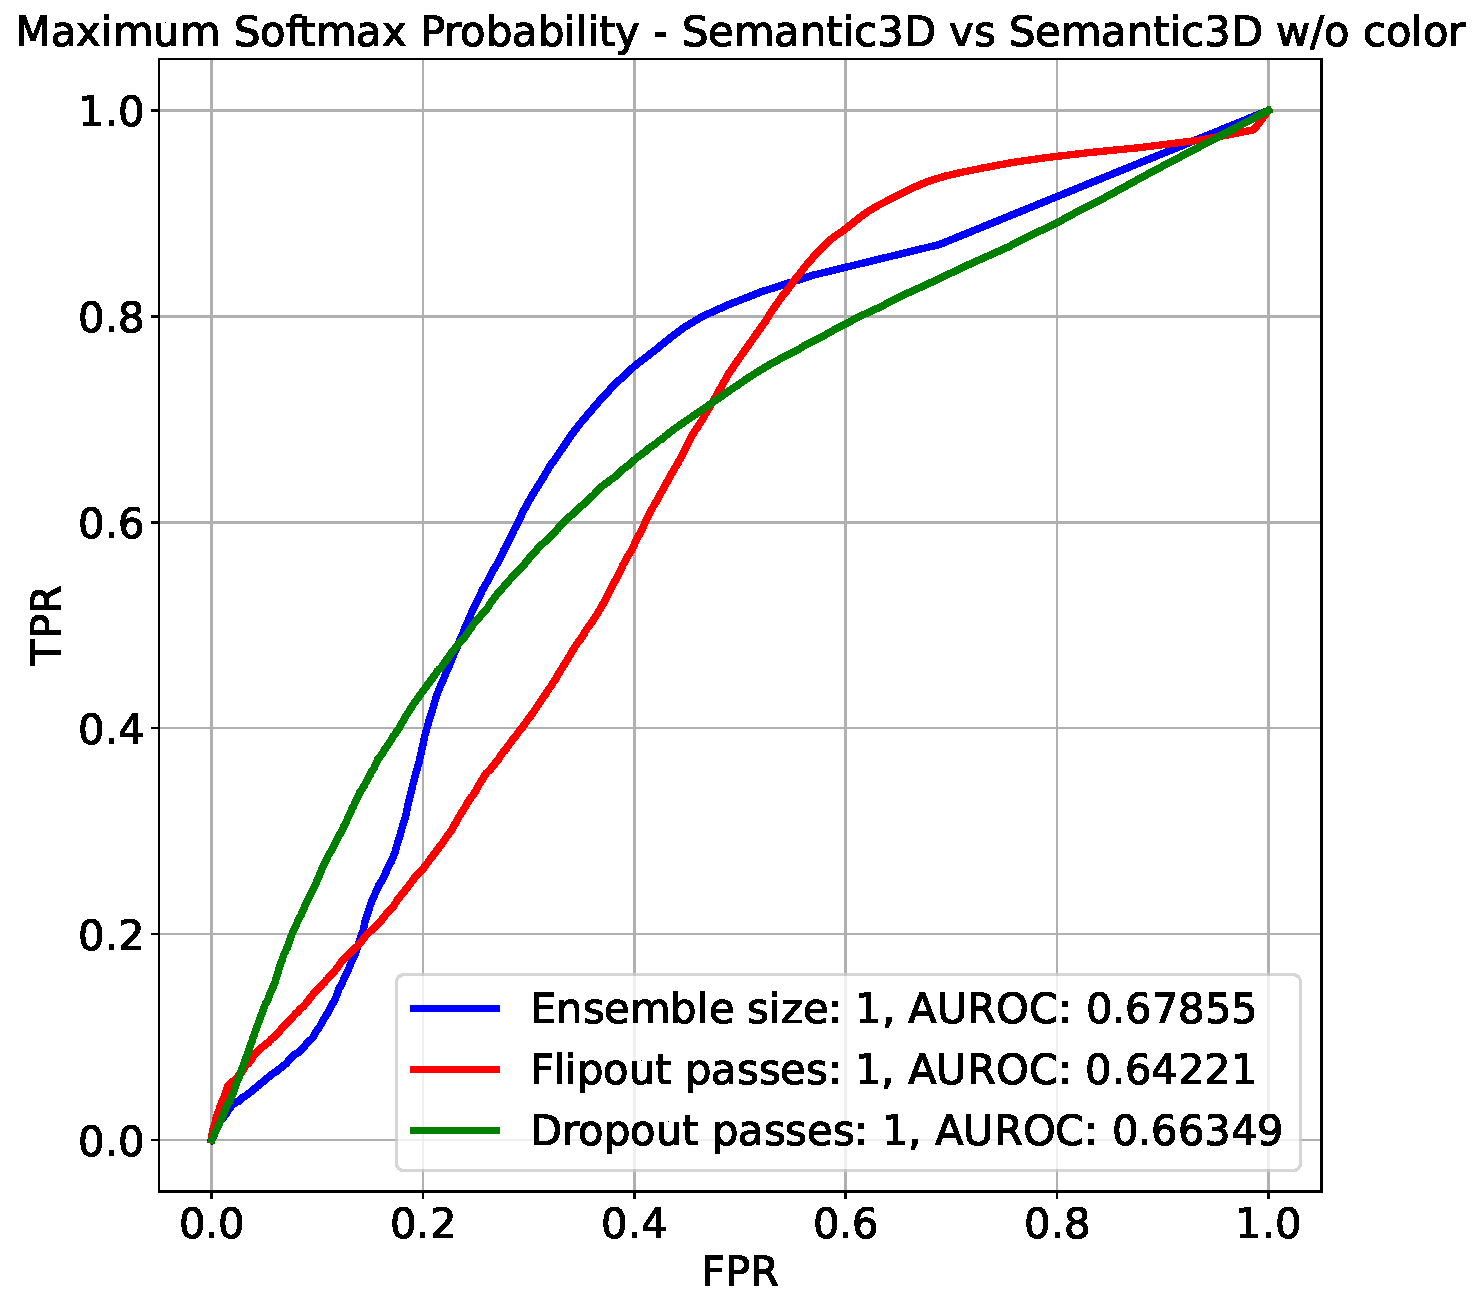
\includegraphics[width = 0.42\textwidth, height= 0.3\textheight]{images/AUROC/MSP_cnc_1.pdf} & 
            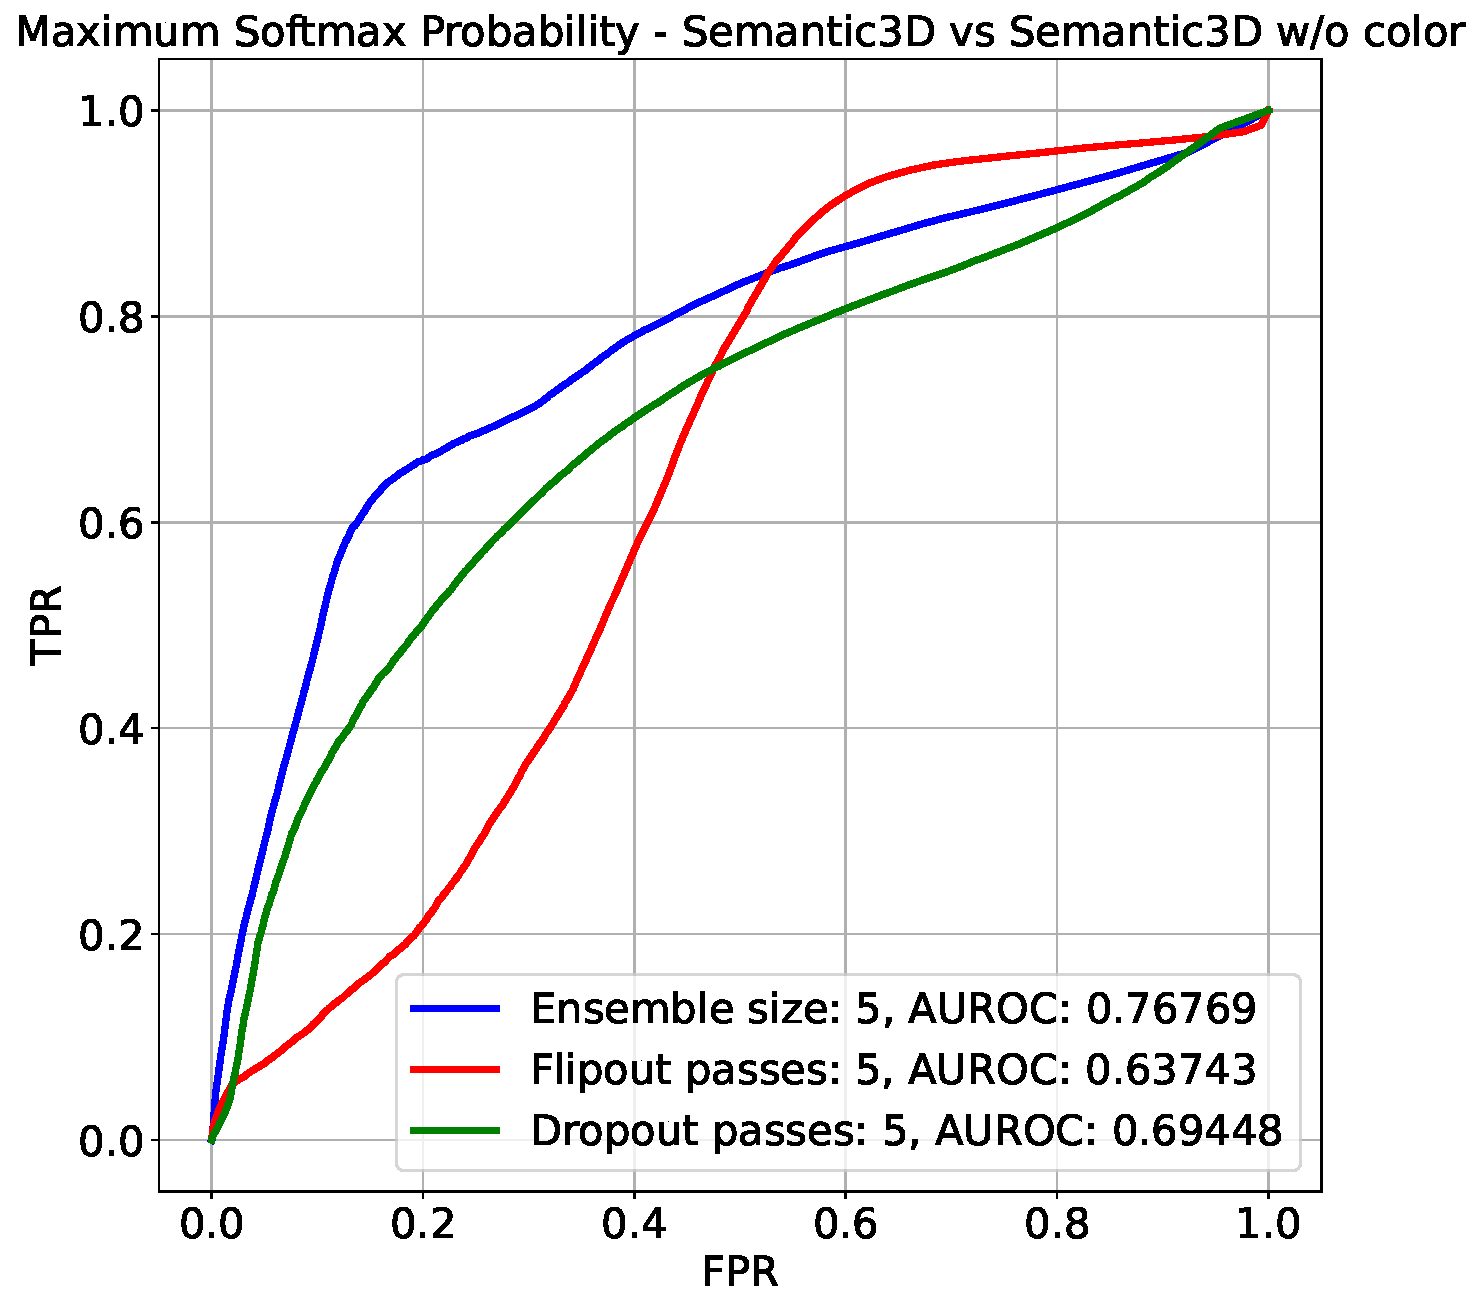
\includegraphics[width = 0.42\textwidth, height= 0.3\textheight]{images/AUROC/MSP_cnc_5.pdf}\\ 
            %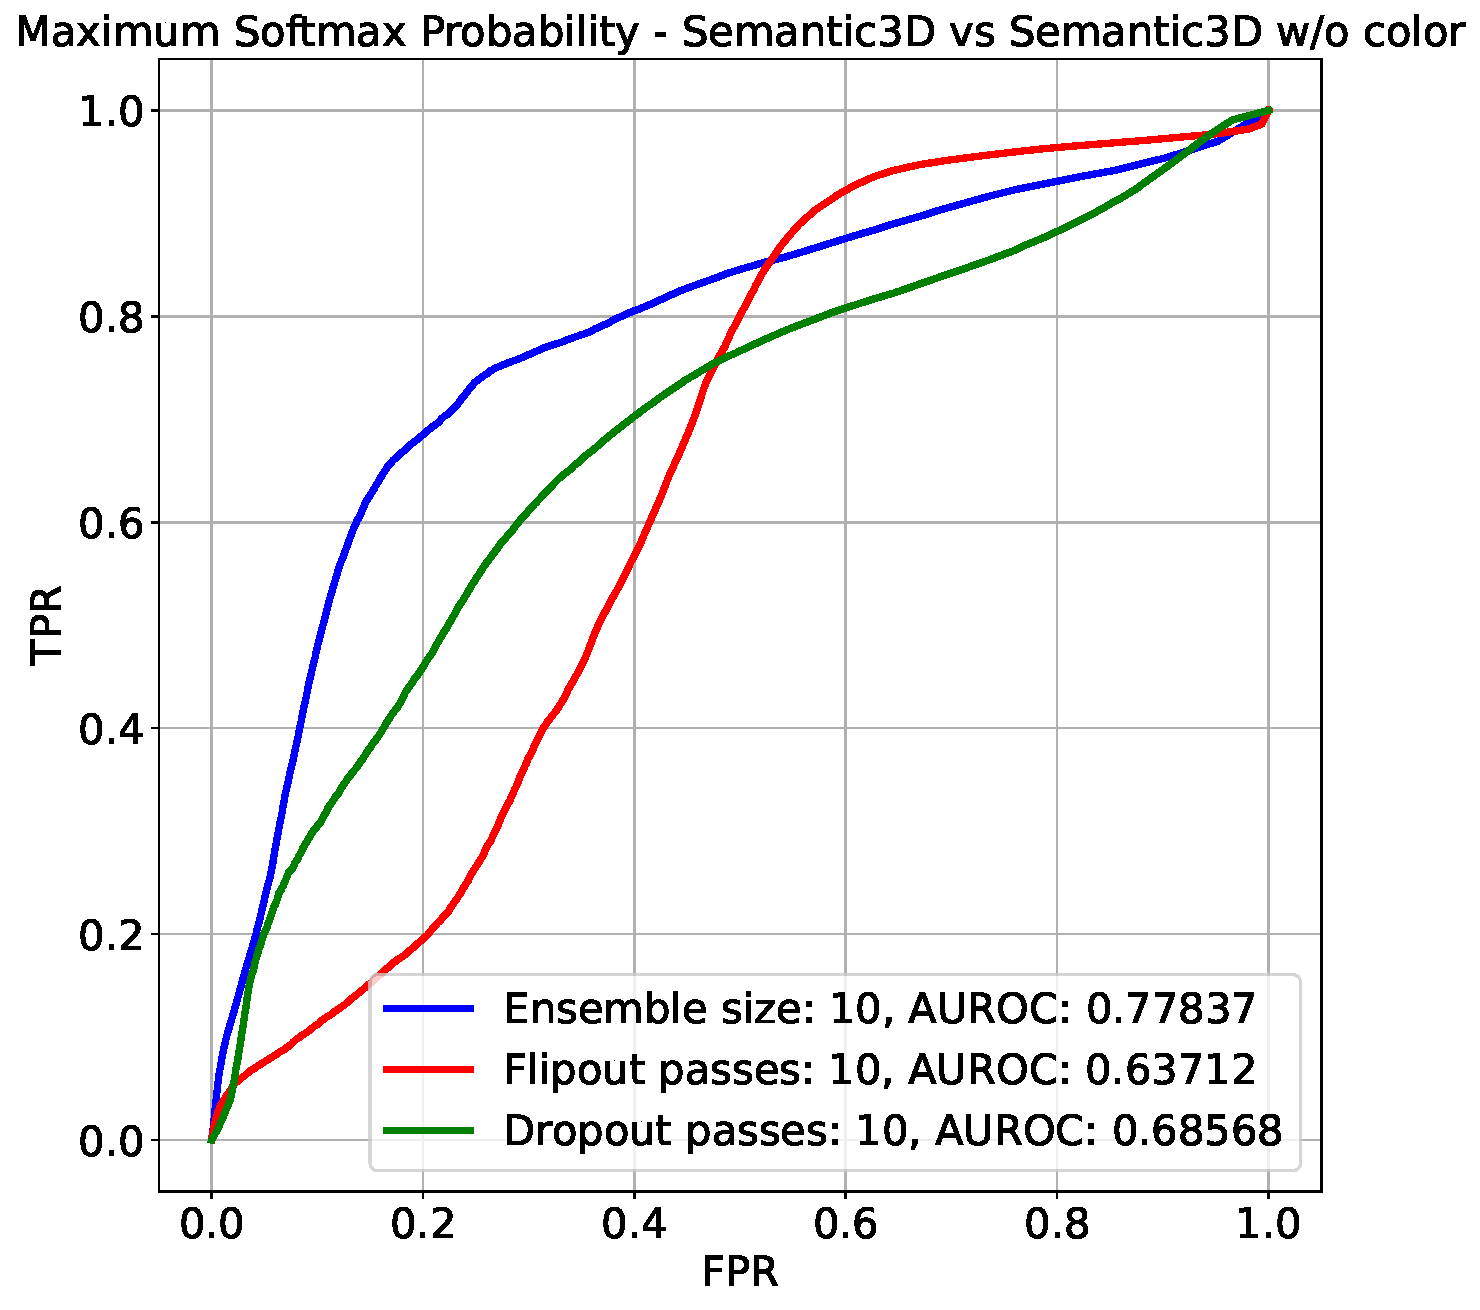
\includegraphics[width = 0.42\textwidth, height= 0.3\textheight]{images/AUROC/MSP_cnc_10.pdf} &
            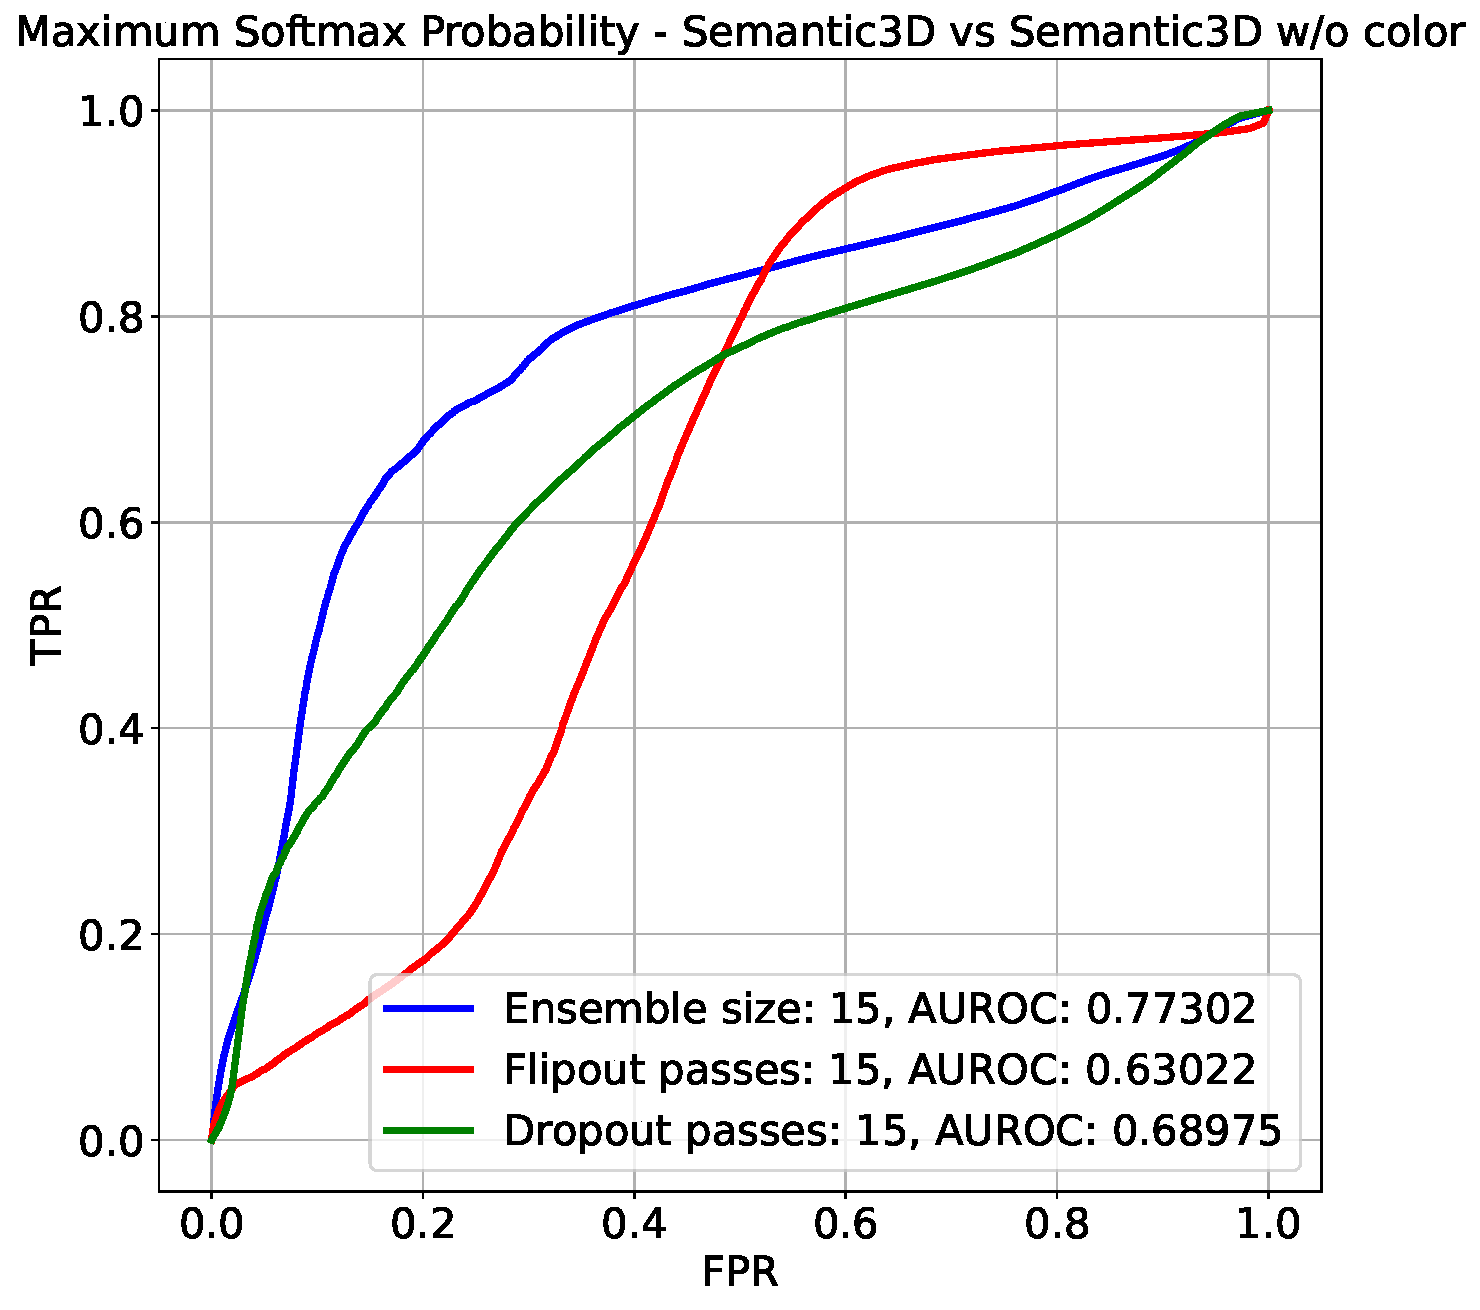
\includegraphics[width = 0.42\textwidth, height= 0.3\textheight]{images/AUROC/MSP_cnc_15.pdf} &
            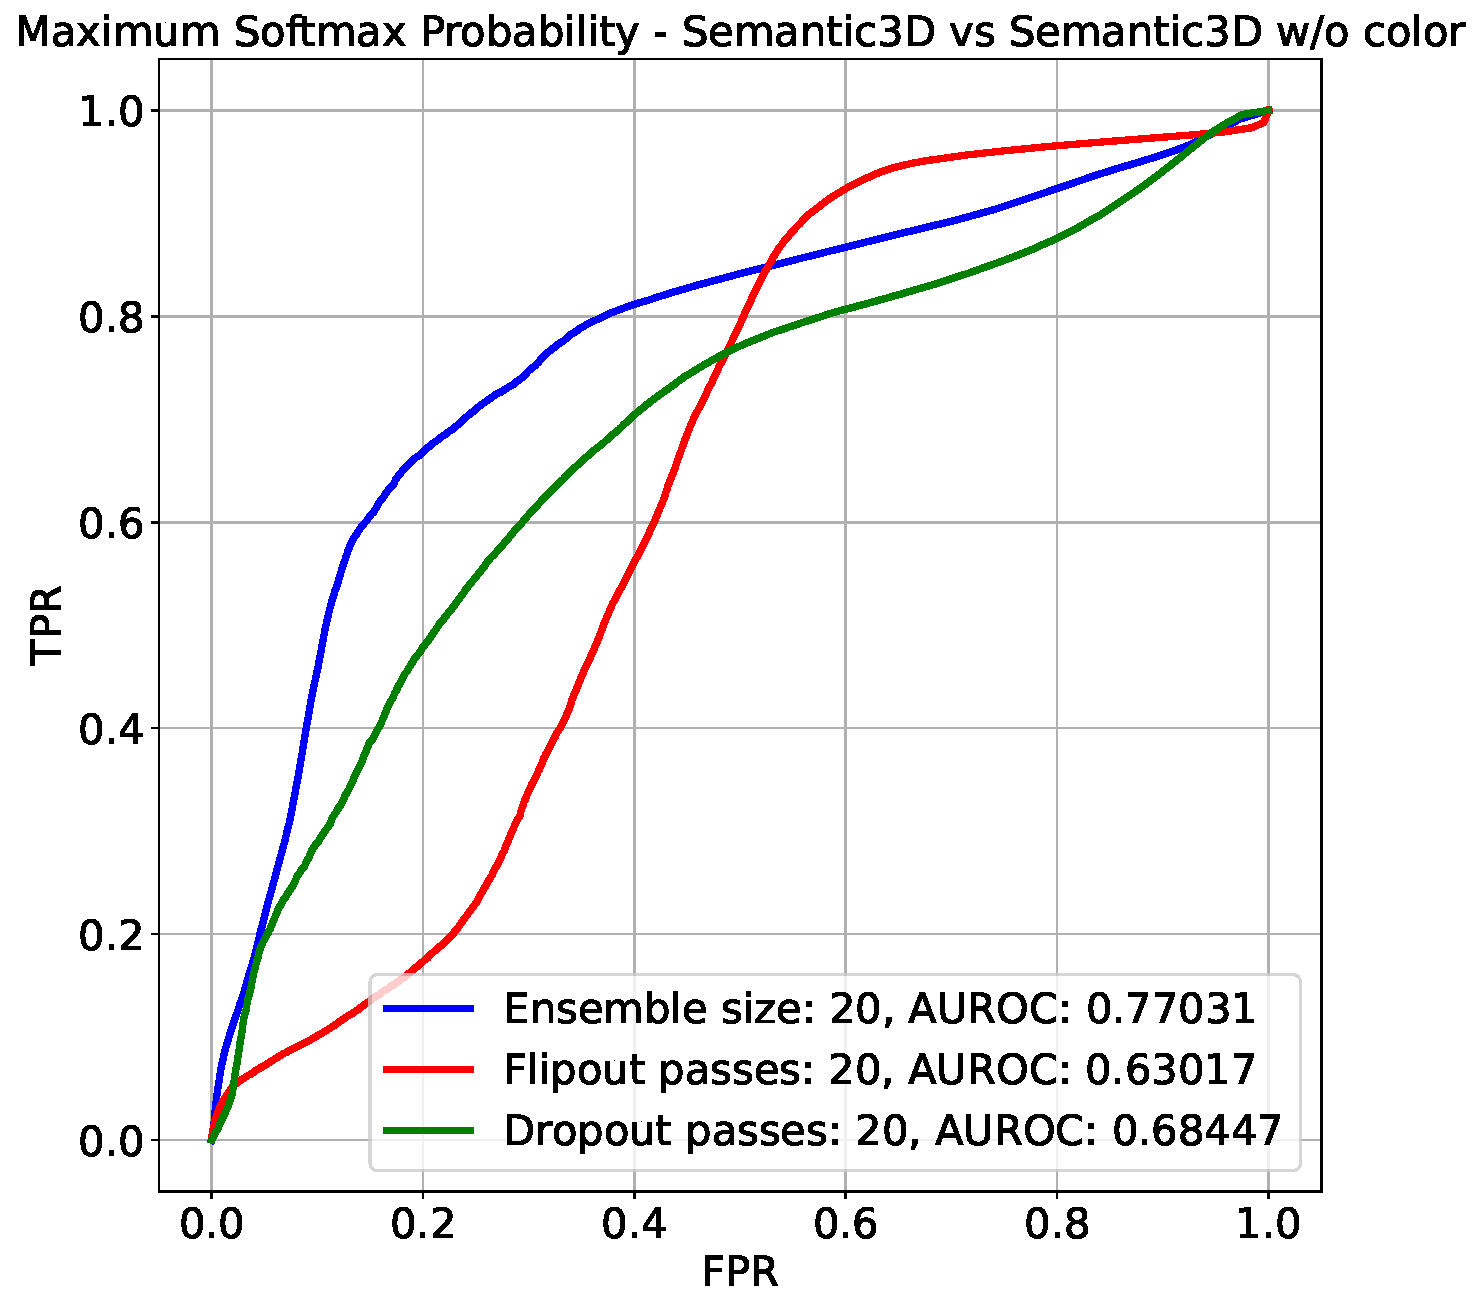
\includegraphics[width = 0.42\textwidth, height= 0.3\textheight]{images/AUROC/MSP_cnc_20.pdf} 
            \\
        \end{tabular}
        \caption{ROC curves for Semantic3D vs Semantic3D without color generated using Maximum Softmax Probability for Deep Ensembles, Flipout and Dropout.}
        \label{fig:roc_msp_ood_2}
    \end{figure*}
    \begin{figure*}
        \centering
        \begin{tabular}{cc}
            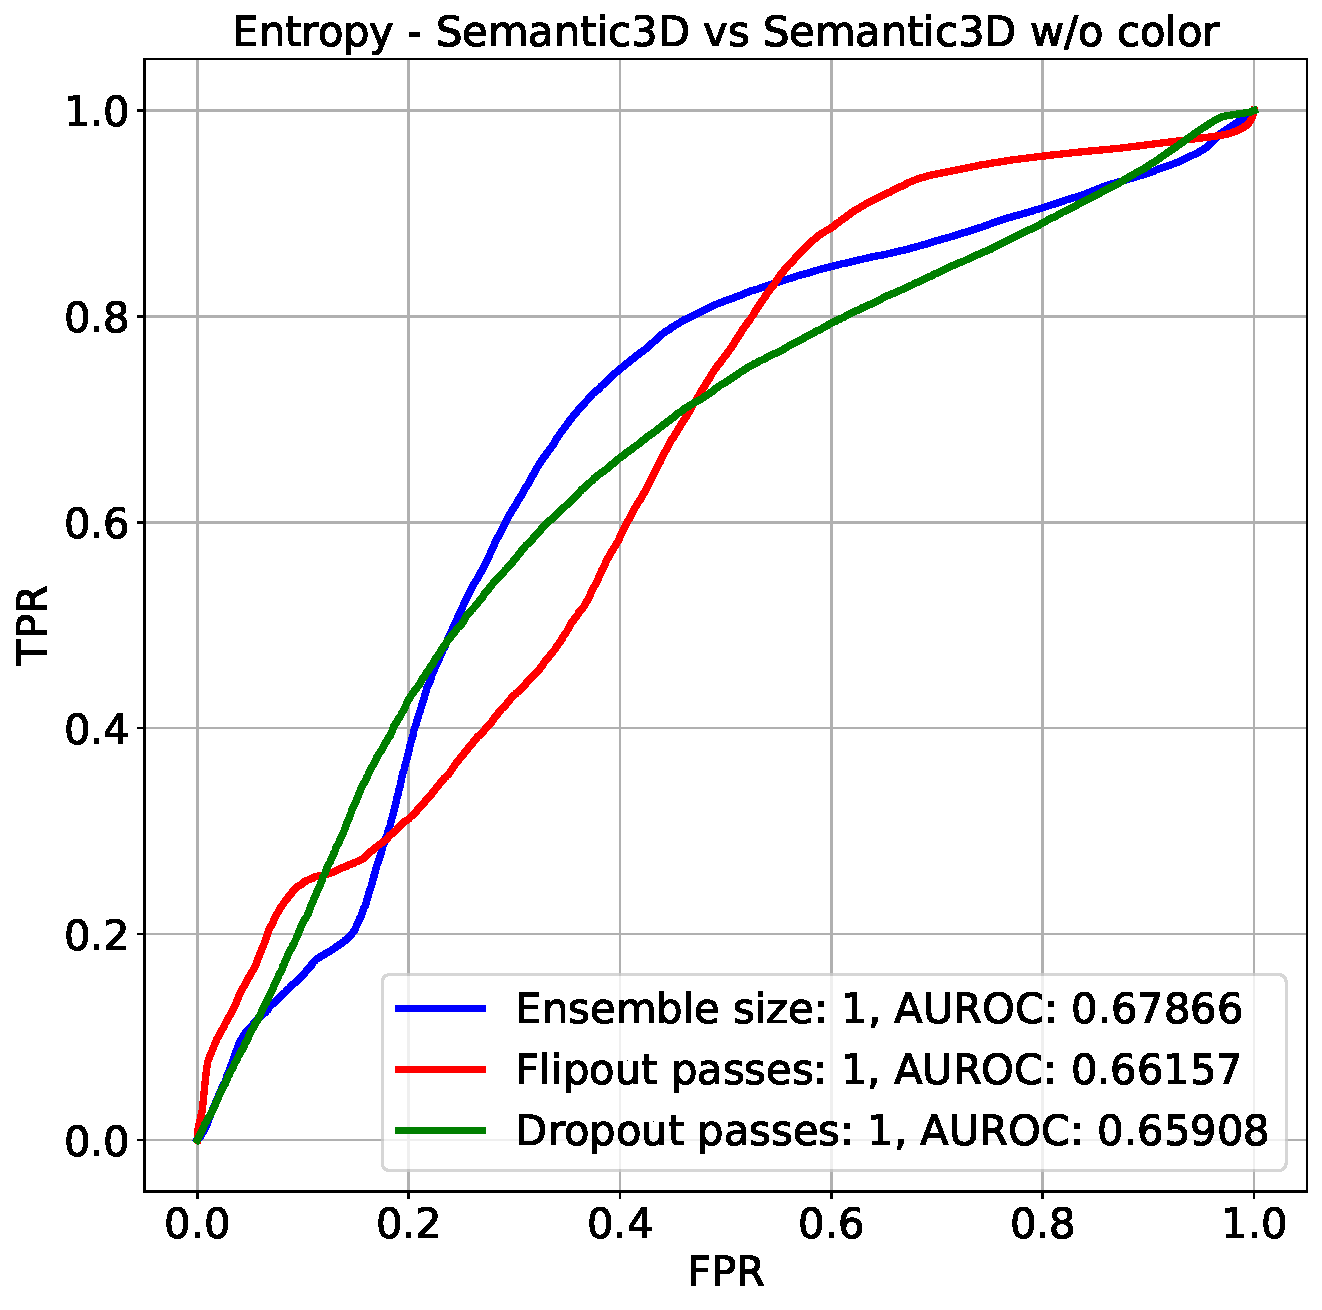
\includegraphics[width = 0.42\textwidth, height= 0.3\textheight]{images/AUROC/Entropy_cnc_1.pdf} & 
            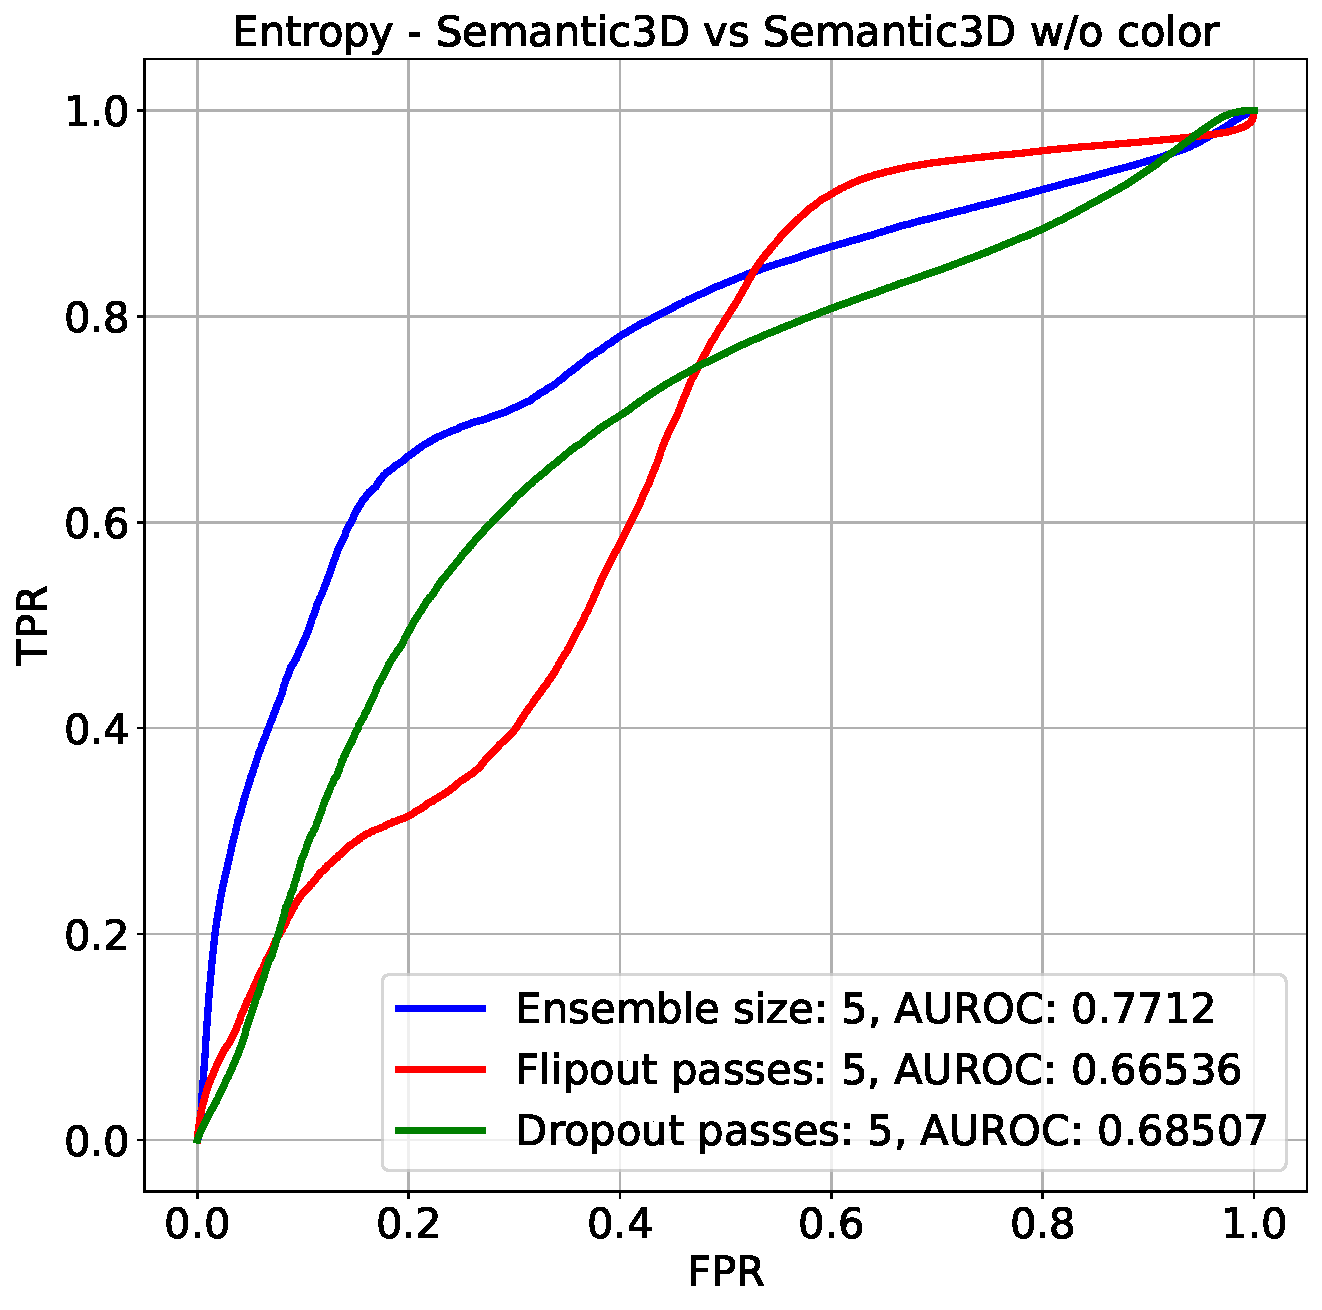
\includegraphics[width = 0.42\textwidth, height= 0.3\textheight]{images/AUROC/Entropy_cnc_5.pdf}\\ 
            %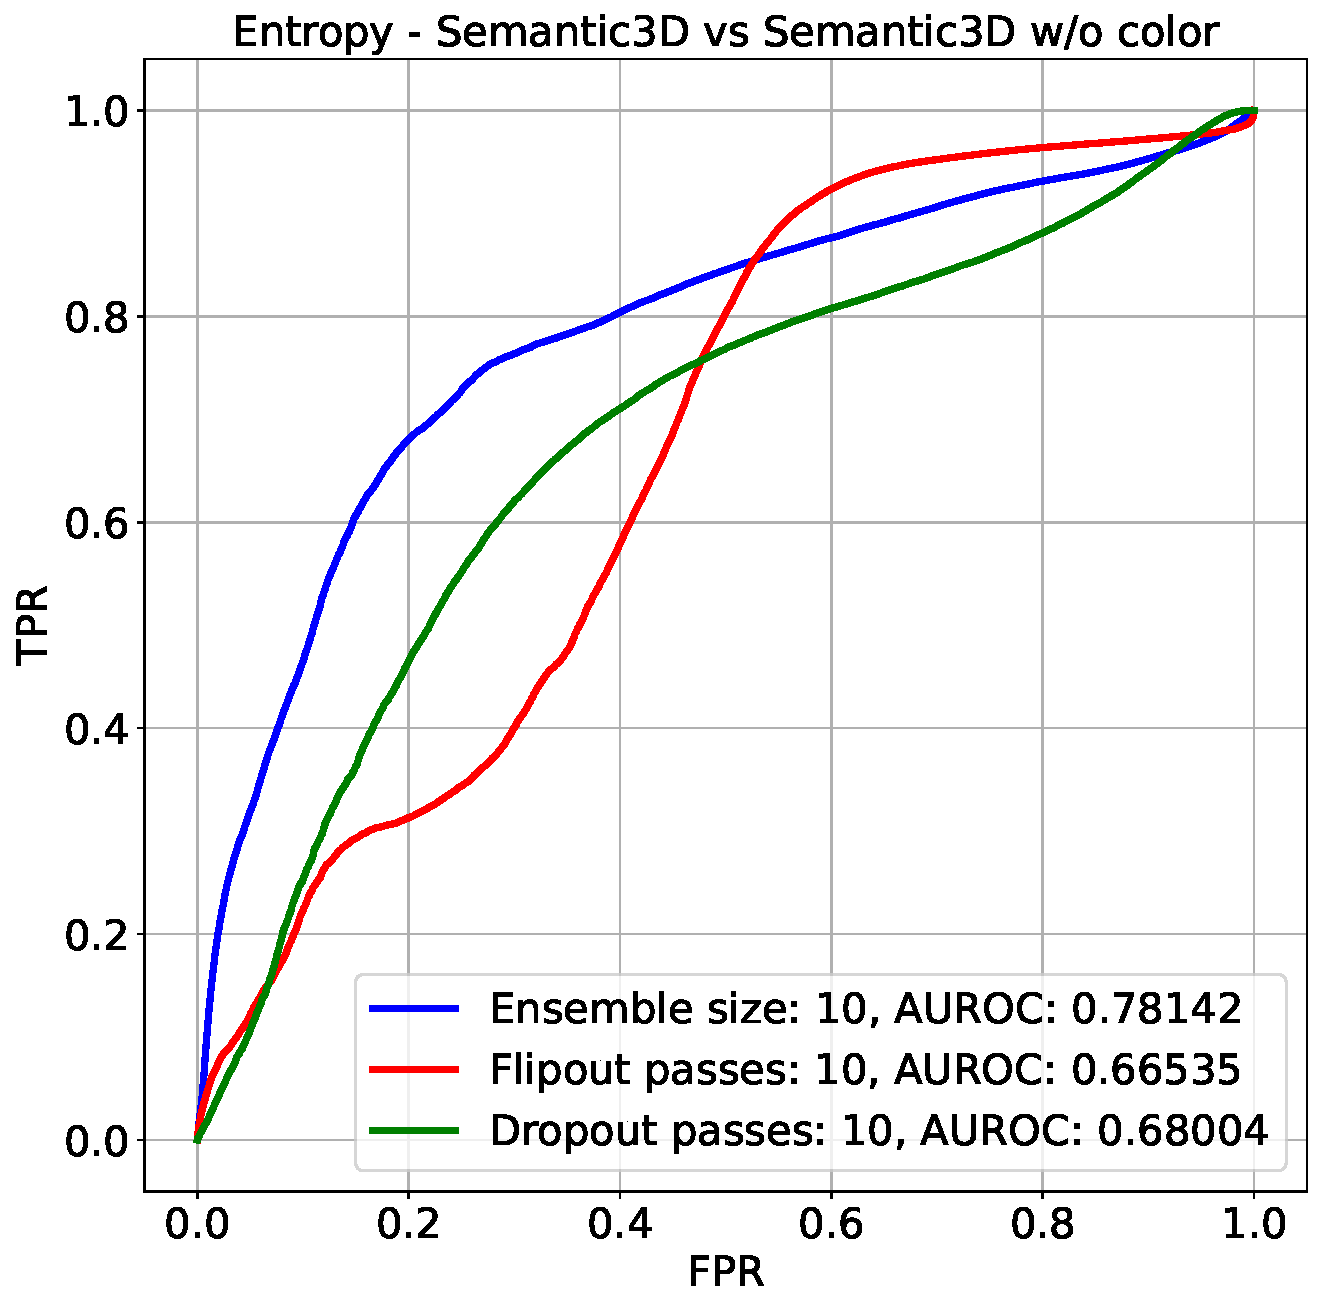
\includegraphics[width = 0.42\textwidth, height= 0.3\textheight]{images/AUROC/Entropy_cnc_10.pdf} &
            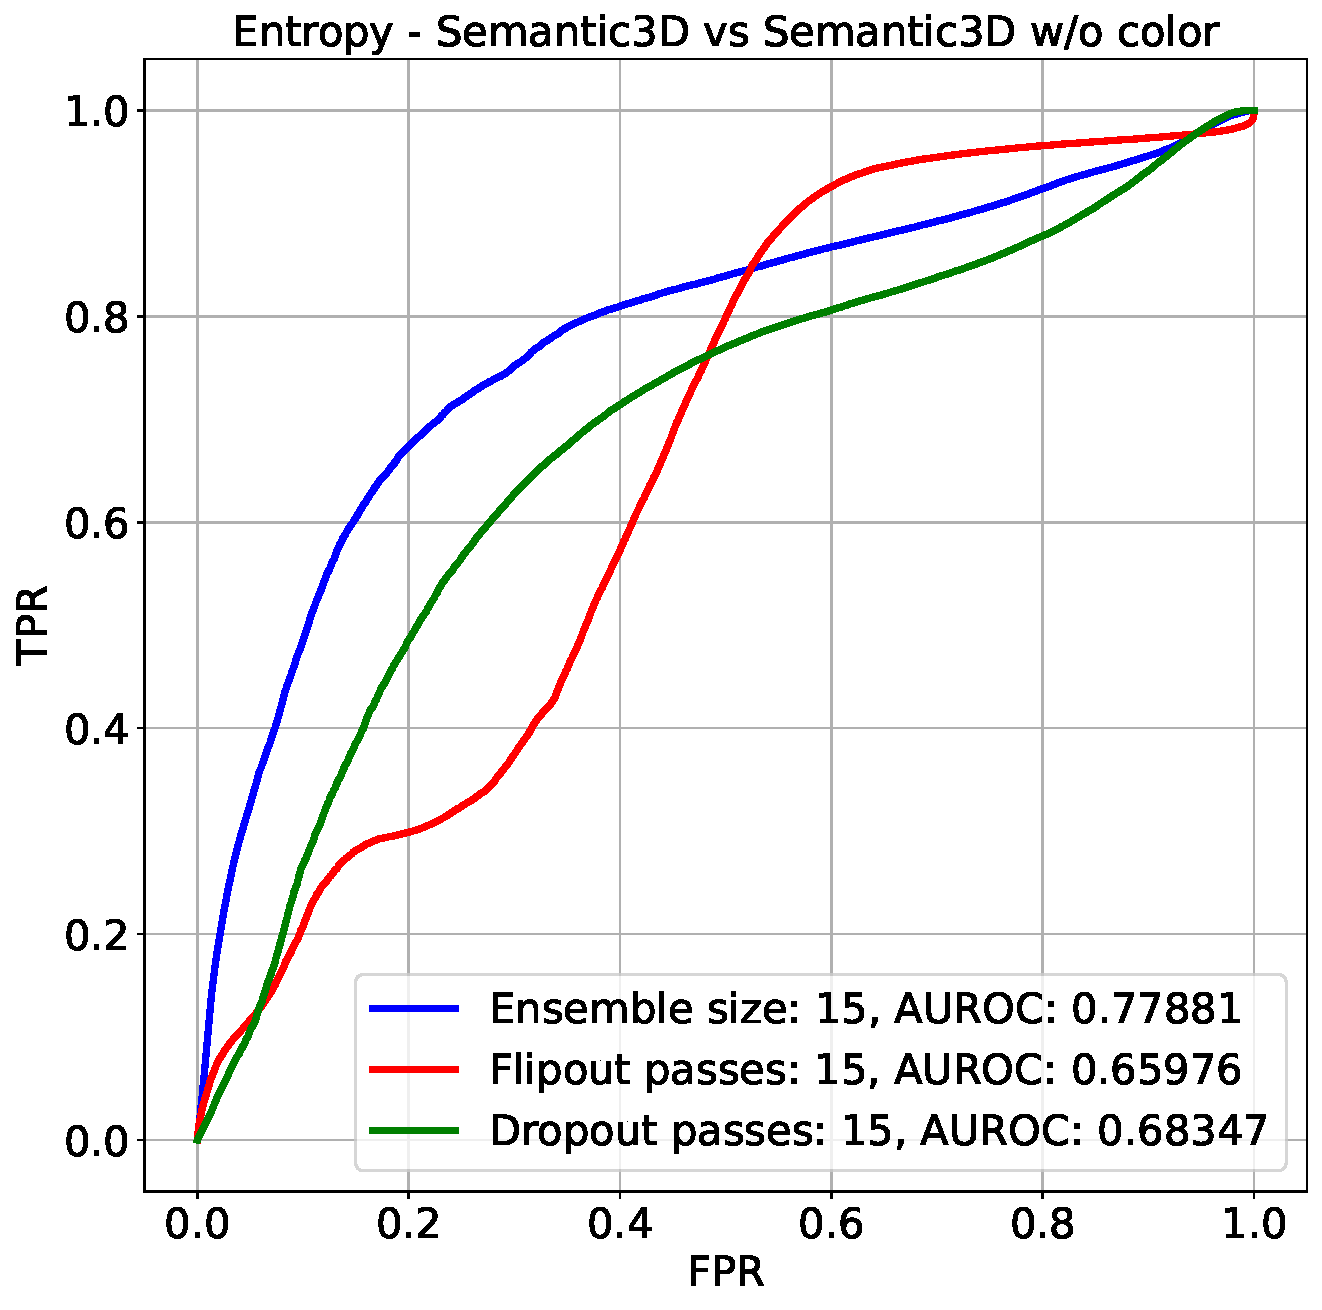
\includegraphics[width = 0.42\textwidth, height= 0.3\textheight]{images/AUROC/Entropy_cnc_15.pdf} &
            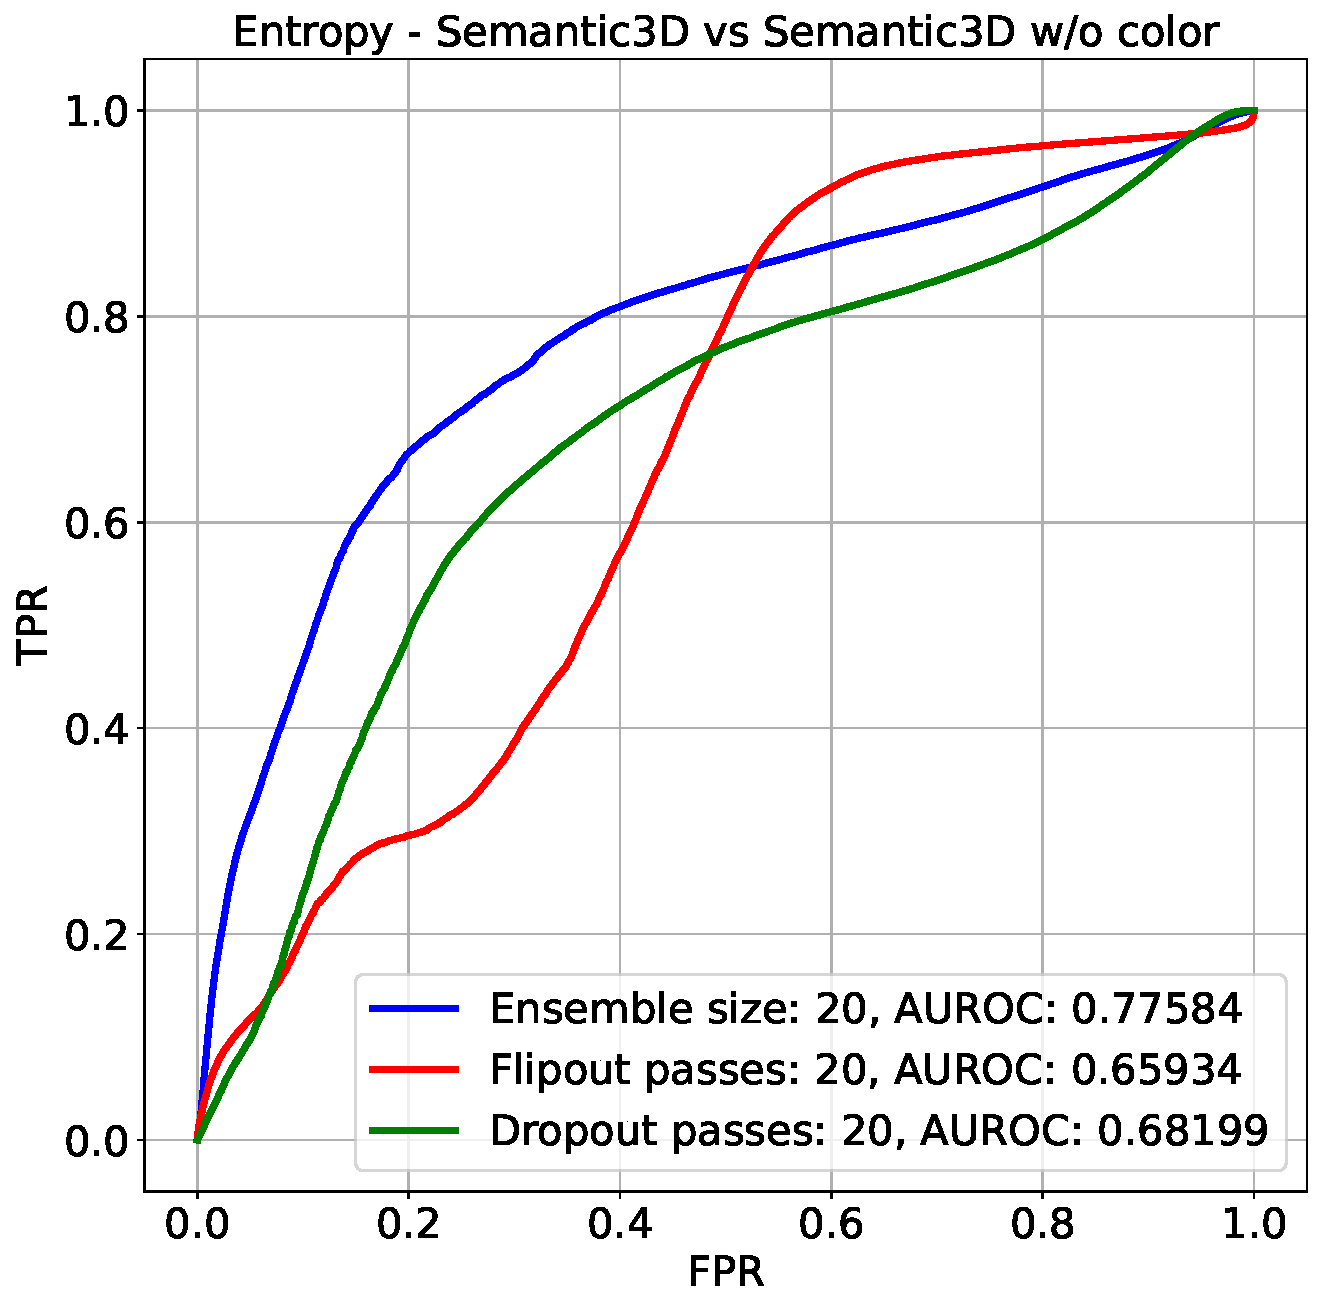
\includegraphics[width = 0.42\textwidth, height= 0.3\textheight]{images/AUROC/Entropy_cnc_20.pdf} 
            \\
        \end{tabular}
        \caption{ROC curves for Semantic3D vs Semantic3D without color generated using Entropy for Deep Ensembles, Flipout and Dropout.}
        \label{fig:roc_ent_ood_2}
    \end{figure*}    
\end{document}
